\documentclass{article}
\usepackage[english]{babel}
\usepackage{geometry,amsmath,amssymb,graphicx,bbm,latexsym,theorem}
\geometry{letterpaper}
\usepackage{geometry,amsmath,amssymb,graphicx,bbm,theorem,xr}

%%%%%%%%%% Start TeXmacs macros
\newcommand{\Nu}{\mathrm{N}}
\newcommand{\assign}{:=}
\newcommand{\comma}{{,}}
\newcommand{\longhookrightarrow}{{\lhook\joinrel\relbar\joinrel\rightarrow}}
\newcommand{\nequiv}{\not\equiv}
\newcommand{\nin}{\not\in}
\newcommand{\nni}{\not\ni}
\newcommand{\nobracket}{}
\newcommand{\nocomma}{}
\newcommand{\nosymbol}{}
\newcommand{\tmmathbf}[1]{\ensuremath{\boldsymbol{#1}}}
\newcommand{\tmop}[1]{\ensuremath{\operatorname{#1}}}
\newcommand{\tmtextbf}[1]{{\bfseries{#1}}}
\newcommand{\tmtextit}[1]{{\itshape{#1}}}
\newcommand{\tmtextrm}[1]{{\rmfamily{#1}}}
\newcommand{\tmtextup}[1]{{\upshape{#1}}}
\newcommand{\um}{-}
\newcommand{\upl}{+}
\catcode`\>=\active \def>{
\fontencoding{T1}\selectfont\symbol{62}\fontencoding{\encodingdefault}}
\newcommand{\tmrsub}[1]{\ensuremath{_{\textrm{#1}}}}
\newcommand{\tmrsup}[1]{\textsuperscript{#1}}
\newenvironment{proof}{\noindent\textbf{Proof\ }}{\hspace*{\fill}$\Box$\medskip}
\newtheorem{definition}{Definition}
\newtheorem{lemma}{Lemma}
\newtheorem{proposition}{Proposition}
{\theorembodyfont{\rmfamily}\newtheorem{remark}{Remark}}
%%%%%%%%%% End TeXmacs macros

\newcommand{\D}{\mathcal{D}}
% 

\newcommand{\supp}{\tmop{supp}}
% 

\newcommand{\proofexplanation}[1]{(#1)}
% 

\newcommand{\C}{\mathbbm{C}}
\newcommand{\Z}{\mathbbm{Z}}
% 

\newcommand{\Sp}{\mathbbm{S}}
% 

\newcommand{\R}{\mathbbm{R}}
% 

\newcommand{\mybra}[1]{(#1)}
% 

\newcommand{\mysbra}[1]{\left[ #1 \right]}
% 

\newcommand{\mycbra}[1]{\left\{#1\right\}}
\newcommand{\sone}{\ensuremath{\mybra{\D' (G \times_P \C_{\lambda - n})
\otimes \C_{\nu}}^{\Delta (P')}}}
\newcommand{\Upp}{{\mysetn{(x,y){\in}{\R}\tmrsup{p,q}}{x{\neq}0,{\hspace{0.75em}}y{\neq}0}}}
\newcommand{\Stab}{O(p,q)\tmrsub{e\tmrsub{p}}}
\newcommand{\sol}{{\sol*{{\R}\tmrsup{p,q}}}}
\newcommand{\solXi}{{\sol*{{\Xi}}}}

\externaldocument{master_master1}
\externaldocument{master_master2}
\externaldocument{master_master3}

\begin{document}

\title{Study of symmetry breaking operators of indefinite orthogonal groups $O( p, q)$.\\ 
IV. Properties of symmetry breaking operators.}
\author{T. Kobayashi, O. Leontiev}
\maketitle
{\tableofcontents}
\setcounter{section}{24}
\section{CAS and related notions}\label{sec:CAS}

\subsection{Main results}

\begin{definition}
  \label{CAS:def-CAS}Let $M$ be a manifold and $R \subset \mathcal{D}' (M)$ is
  a linear subspace. We say \tmtextbf{$R$ is a CAS} (abbreviation for
  ``Closed, Approximable by Smooth'') if the following holds:
  \begin{enumerate}
    \item for every $f \in R$ there exist $f_n \in C^{\infty} (M) \cap R$ such
    that $f_n \rightarrow f$ in $\mathcal{D}' (M)$;
    
    \item whenever $f_n \in R$ converges (in $\mathcal{D}' (M)$) to some $f
    \in \mathcal{D}' (M)$, we have $f \in R$.
  \end{enumerate}
\end{definition}

\begin{definition}
  \label{CAS:def-map}Let $M, M'$ be manifolds with $R, R'$ the respective
  CAS's and $F : C^{\infty} (M) \cap R \rightarrow C^{\infty} (M') \cap R'$ be
  a linear map. We say $F$ \tmtextbf{induces map between CAS} if whenever $R
  \cap C^{\infty} (M) \supset \{ f_n \}_{n = 1}^{\infty}$ converges, so does
  $F (f_n)$ and if $R \cap C^{\infty} (M) \ni f_n \rightarrow 0$, then $F
  (f_n) \rightarrow 0$.
  
  If $F$ has an inverse $F^{- 1} : C^{\infty} (M') \cap R' \rightarrow
  C^{\infty} (M) \cap R$ that also induces map between CAS, we say $F$
  \tmtextbf{\tmtextit{induces isomorphism between CAS}}.
\end{definition}

\begin{remark}
  Note the following:
  \begin{enumerate}
    \item definition of CAS implies that there exists $F' : R \rightarrow R'$
    such that $F' \big|_{C^{\infty} (M) \cap R} = F$ and $R \ni f_n
    \rightarrow f \in R$ implies $R' \ni F' (f_n) \rightarrow F' (f) \in R'$
    (we simply define $F'$ by limits). Such $F'$ is called \tmtextbf{map
    between CAS}. In case $F$ induces isomorphism, induced $F'$ is called
    \tmtextbf{isomorphism between CAS}.
    
    \item definition of CAS implies that extension $F' : R \rightarrow R'$ is
    unique;
    
    \item it is trivial to observe that if $F$ induces isomorphism between
    CAS, then its extension $F' : R \rightarrow R'$ is isomorphism of vector
    spaces.
    
    \item CAS form a category;
  \end{enumerate}
\end{remark}

\begin{proposition}
  \label{CAS:prop-GoverP}Let $G$ be a Lie group with $H \subset G$ closed
  subgroup and $\rho : H \curvearrowright \mathbbm{C}$ its representation.
  Then $\mathcal{D}' (G)_H \assign \left\{ f \in \mathcal{D}' (G) \big|
  \forall h \in H, \; f (\cdot h) = \rho (h) f (\cdot) \right\} \subset
  \mathcal{D}' (G)$ is a CAS and a projection map $C^{\infty} (G)_H
  \rightarrow C^{\infty} (G / H, G \times_H \rho)$ induces isomorphism
  $\mathcal{D}' (G)_H \rightarrow \mathcal{D}' (G / H, G \times_H \rho)$
  between CAS.
\end{proposition}

\begin{proposition}
  \label{CAS:prop-GoverP-holo}Suppose $G$ is a Lie group and $H \subset G$ is
  its closed subgroup. Then, proposition \ref{CAS:prop-GoverP} implies that we
  have a CAS isomorphism $\mathcal{D}' (G)_H \assign \left\{ \mathcal{D}' (G)
  \big| \forall h \in H, \; f (\cdot h) = f (\cdot) \right\}
  \tilde{\rightarrow} \mathcal{D}' (G / H)$. Suppose further that $f_{\mu} \in
  \mathcal{D}' (G / H)$ is holomorphic in $\mu \in \Omega$, where $\Omega
  \subset \mathbbm{C}^m$ is open set. We then have preimage $F_{\mu} \in
  \mathcal{D}' (G / H)$ being holomorphic as well.
\end{proposition}

\begin{remark}
  Vector-valued version of this proposition also holds with proof being the
  same (with obvious modifications).
\end{remark}

\begin{proposition}
  \label{CAS:prop-invariant}Suppose $R \subset C^{\infty} (M)$ and $R' \subset
  C^{\infty} (M')$ are CAS with $F : C^{\infty} (M) \cap R \rightarrow
  C^{\infty} (M') \cap R'$ inducing a map between CAS. Suppose further that
  $\{ F_i : C^{\infty} (M) \cap R \rightarrow C^{\infty} (M) \cap R \}_{i \in
  I}$ and $\{ F'_i : C^{\infty} (M') \cap R' \rightarrow C^{\infty} (M') \cap
  R' \}_{i \in I}$ are two families that induce isomorphism of CAS's, indexed
  by the same index set $I$ such that the following diagram commutes for every
  $i \in I$:
  \begin{center}
    \resizebox{0.7\columnwidth}{!}{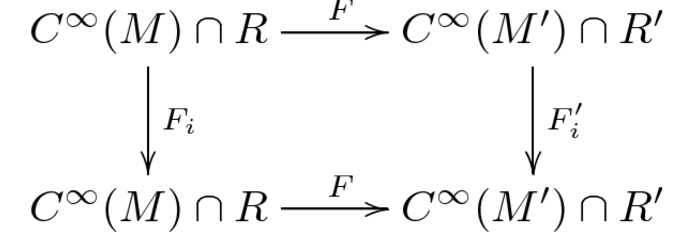
\includegraphics{master_master-11.png}}
    
    \ 
  \end{center}
  Then, (extending $F$, $\{ F_i \}_i$ and $\{ F_i' \}_i$ to maps between CASs
  as in remark after definition \ref{CAS:def-map}) restriction of $F$ induces
  a linear map $R^{\{ F_i \}_i} \rightarrow R^{\prime\{ F_i' \}_i}$, where
  $R^{\{ F_i \}_i} \assign \left\{ f \in R \big| \forall i \in I, \; F_i
  (f) = f \right\}$ and $R^{\prime\{ f_i' \}_i}$ is similarly defined.
  Moreover, if $F$ was an isomorphism between CAS, then the induced map is
  also an isomorphism of vector spaces.
\end{proposition}

\begin{proposition}
  \label{CAS:prop-restriction}Suppose $G$ is Lie group with $P, H \subset G$
  closed subgroups such that $P H = G$ and $H_P \assign P \cap H$. We also
  assume we have representation $\rho : P \rightarrow \tmop{GL}^1
  (\mathbbm{C})$. We then have pullback
  \begin{eqnarray}
    & C^{\infty} (G)_P \assign \{ f \in C^{\infty} (G) | \forall p \in P, f
    (\cdot p) = \rho (p) f (\cdot) \} \rightarrow C^{\infty} (H)_{H_P} \assign
    \{ f \in C^{\infty} (H) | \forall p \in H_P, f (\cdot p) = \rho (p) f
    (\cdot) \} &  \nonumber
  \end{eqnarray}
  induced by $H \longhookrightarrow G$ inclusion inducing map of CAS,
  $\mathcal{D}' (G)_P \rightarrow \mathcal{D}' (H)_{H_P}$. Moreover, there
  exists closed cone $\Gamma \subset G$ such that $\Gamma \cap N_{H \subset G}
  = \varnothing$ (with $N_{H \subset G}$ denoting normal bundle) and
  $\mathcal{D}' (G)_P \subset \mathcal{D}' (G)_{\Gamma}$. The pullback of
  distribution then gives the $\mathcal{D}' (G)_P \rightarrow \mathcal{D}'
  (H)_{H_P}$ map, which is a map of CAS.
\end{proposition}

\begin{proposition}
  \label{CAS:prop-proj}Let $G, H$ be Lie groups and $\rho : H \mapsto
  \tmop{GL} (\mathbbm{C}^1)$ be a representation of $H$. We then have the map
  \[ \mathcal{D}' (G) \ni f \mapsto f \otimes \rho \in \mathcal{D}' (G \times
     H)_H \assign \left\{ g \in \mathcal{D}' (G \times H) \big| \forall h
     \in H, \; g (\cdot, \cdot h) = \rho (h) g (\cdot, \cdot) \right\} \]
  being an isomorphism of CAS.
\end{proposition}

\subsection{Auxiliary lemmas}

\begin{lemma}
  \label{CAS:lem-aux}Suppose $G$ is a Lie group, $H$ is its closed subgroup
  $\rho : H \rightarrow \tmop{GL} (\mathbbm{C}^1)$ is a (Lie group)
  representation and $\mathcal{D}' (G)_H \assign \{ f \in \mathcal{D}' (G) |
  \forall h \in H, f (\cdot h) = \rho (h) f (\cdot) \}$. We further let for $g
  \in G$ the $V_g \subset T^{\ast}_g G$ be fiber at $g$ of normal bundle of
  submanifold $H \ni h \mapsto g h \in G$ of $G$. Then, we let $\Gamma \assign
  \{ (g, V_g) | g \in G \}$: closed conic subset of $T^{\ast} G$. Then,
  $\mathcal{D}' (G)_H \subset \mathcal{D}'_{\Gamma} (G)$ and moreover if
  $\varphi_n \in \mathcal{D}' (G)_H$ converges in $\mathcal{D}' (G)$, it also
  does so in $\mathcal{D}'_{\Gamma} (G)$.
\end{lemma}

\begin{proof}
  {\cite[thm. 8.3.1]{hormander1983analysis}} readily implies the first
  conclusion of the result. To prove the second, we take sequence
  $\mathcal{D}' (G)_H \ni \varphi_n$ that converges in $\mathcal{D}' (G)$.
  Now, we let $\mathfrak{h} \subset \mathfrak{g}$ be Lie algebras of $G$ and
  $H$ respectively and let $\mathfrak{a}$ be some complement of $\mathfrak{h}$
  in $\mathfrak{g}$, so that $\mathfrak{g} \simeq \mathfrak{h} \oplus
  \mathfrak{a}$ and $\mathfrak{g}^{\ast} \simeq \mathfrak{h}^{\ast} \oplus
  \mathfrak{a}^{\ast}$.
  
  We now have for every $g_0 \in G$ map $\mathfrak{a} \times H \ni (X, h)
  \mapsto g_0 \exp (X) h \in G$ be diffeomorphism near $(0, 1)$ by inverse
  function theorem, hence we can pullback some neighborhood $U$ of $g_0$ to
  $\mathfrak{a} \times H \supset V \times O \ni (0, 1)$. Pulling the
  (restriction to $U$) of $\varphi_n$ to $V \times O$ we get $\psi_n \in
  \mathcal{D}' (V \times O)$ and $H$-invariance together with fact
  \ref{fact:sing-q-4} imply that $\psi_n = \phi_n \otimes \psi \in
  \mathcal{D}' (V) \otimes C^{\infty} (O)$ and hence $\psi_n \in \mathcal{D}'
  (V)$ is convergent. Therefore, fact \ref{holomorphicity-preserving:fact-p1}
  implies that $\psi_n$ is convergent in $\mathcal{D}'_{\Gamma_1 \otimes
  \Gamma_2}$ where $\Gamma_1$ is full cone in $\mathfrak{a}$, while $\Gamma_2$
  is zero cone in $H$ and $\otimes$ is as in fact
  \ref{holomorphicity-preserving:fact-p1}. Now, inspecting how $\otimes$ was
  defined, we see that after pulling back $\Gamma_1 \otimes \Gamma_2$ to $G$
  via diffomorphism $U \simeq V \times O$, we have that it becomes exactly as
  claimed in the statement.
\end{proof}

\subsection{Proofs}

\begin{proof}
  (of proposition \ref{CAS:prop-GoverP}) We note that as $\pi : G \rightarrow
  G / H$ is a principal bundle, we can cover $G / H$ with open cover $\{ U_i
  \}_i$ and have diffeomorphisms $\psi_i : \pi^{- 1} (U_i) \tilde{\rightarrow}
  U_i \times H$. We also have transition cocycles $\gamma_{i, j} : U_{i, j}
  \assign U_i \cap U_j \rightarrow H$, so that for $x \in U_{i, j}$ we have
  $\psi_j (x) = (\tmop{id}_{U_{i, j}} \times \gamma_{i, j} (x)) (\psi_i (x))$.
  
  We first describe a mapping $\mathcal{D}' (G)_H \rightarrow \mathcal{D}' (G
  / H, G \times_H \rho)$. Let $f \in \mathcal{D}' (G)_H$, we let $f_i \in
  \mathcal{D}' (U_i \times H)$ defined by $f_i \assign (\psi_i^{- 1})^{\ast} f
  \big|_{\pi^{- 1} (U_i)}$. As $f \in \mathcal{D}'  (G)_H$, we should have
  $f_i (\cdot, h) = \rho (h) f_i (\cdot, 1)$, hence (slight generalization of)
  fact \ref{fact:sing-q-4} implies that $f_i = g_i \otimes \rho (\cdot)$ with
  $g_i \in \mathcal{D}' (U_i)$ and we define $g \in \mathcal{D}' (G / H, G
  \times_H \rho)$ via the rule $g \big|_{U_i} = g_i$ Here we use the
  (slight generalization of) fact \ref{fact:localization}, so we need to check
  that on $U_{i, j} \assign U_i \cap U_j$ we have $g_j = \rho (\gamma_{i, j})
  g_i$. But this definitely holds, as on $U_{i, j}$ we must have $f_i = f_j$
  (as both were defined by restrictions), hence $g_i \otimes \pi (\cdot) =
  \psi_i \psi_j^{- 1} (g_i \otimes \rho (\cdot))$ and as we've seen before
  $\psi_j \psi_i^{- 1} = \tmop{id}_{U_{i, j}} \times \gamma_{i, j}$, hence
  $g_i \otimes \pi (\cdot) = g_j \otimes \rho (\gamma_{i, j}^{- 1}) \rho
  (\cdot)$, thus $g_j = \rho (\gamma_{i, j}) g_i$ as was required. Thus $g \in
  \mathcal{D}' (G / H, G \times_H \rho)$ is well-defined and the map $F :
  \mathcal{D}' (G)_H \rightarrow \mathcal{D}' (G / H, G \times_H \rho)$ is
  easily seen to be linear, well-defined and sending $C^{\infty} (G)_H$ to
  $C^{\infty} (G / H, G \times_H \rho)$. The construction also implies that if
  $\mathcal{D}' (G)_H \ni f_n \rightarrow f \in \mathcal{D}' (G)_H$, then $F
  (f_n) \rightarrow F (f)$ (one just proves this when restricted to every
  $U_i$) and that if $\mathcal{D}' (G)_H \ni f_n \rightarrow 0$, then $F (f_n)
  \rightarrow 0$ (again, this is proven for every $U_i$).
  
  We then describe the inverse map $F^{- 1} : \mathcal{D}' (G / H, G \times_H
  \rho) \rightarrow D'  (G)_H$. Indeed, with notations as in previous
  paragraph, we take for $g \in \mathcal{D}' (G / H, G \times_H \pi)$ $g_i
  \assign g \big|_{U_i}$ and $f_i \assign g_i \otimes \rho (\cdot) \in
  \mathcal{D}' (U_i \times H)$. The computations of previous paragraph imply
  that $f_i$ patch up to give $f \in \mathcal{D}' (G)_H$ and this map is
  linear inverse to $F$ that takes $C^{\infty} (G / H, G \times_H \rho)$ to
  $C^{\infty} (G)_H$ and such that $\mathcal{D}' (G / H, G \times_H \rho) \ni
  g_n \rightarrow g \in \mathcal{D}' (G / H, G \times_H \rho)$ implies $F^{-
  1} (g_n) \rightarrow F^{- 1} (g)$ and $g_n \rightarrow 0$ implies $F^{- 1}
  (g_n) \rightarrow 0$.
  
  We now prove that $\mathcal{D}' (G)_H \subset \mathcal{D}' (G)$ is a CAS. We
  check the axioms of CAS, starting from the first one. Let $f \in
  \mathcal{D}' (G)_H$, we need to find $f_n \in C^{\infty} (G)_H$ such that
  $f_n \rightarrow f$. Now, we take $g \assign F (f) \in \mathcal{D}' (G / H,
  G \times_H \rho)$ and take $g_n \in C^{\infty} (G / H, G \times_H \rho)$
  such that $g_n \rightarrow g$ (we briefly explain why such construction is
  possible: we can define for every $i$ $\{ g_n^{(i)} \in C^{\infty}_0 (U_i)
  \subset C^{\infty}_0 (G / H, G \times_H \rho) \}_n$ such that $g_n^{(i)}
  \rightarrow g \big|_{U_i}$; and then use $\{ \varphi_i \in C^{\infty} (G
  / H, G \times_H \rho) \}$ partition of unity relative to $U_i$ and define
  $g_n \assign \sum_i g^{(i)_{}}_n \varphi_i$).
  
  We then take $f_n \assign F^{- 1} (g_n) \in C^{\infty} (G)_H$, so that $f_n
  \rightarrow f$. This proves the first axiom of CAS. Second axiom is proven
  as follows: if $\mathcal{D}'  (G)_H \ni f_n \rightarrow f \in \mathcal{D}'
  (G)_H$, then for every $i$, $f_n \big|_{\pi^{- 1} (U_i)}$ converges and
  considerations above (and continuity of pullback) imply that $f_n =
  g_i^{(n)} \otimes \rho \in \mathcal{D}' (U_i \times H)$ converges, and one
  then concludes that $\{ g_i^{(n)} \}_n$ also converges to limit $g_i \in
  \mathcal{D}' (U_i)$. Continuity of operations involved then implies that
  $g_j = \rho (\gamma_{i, j}) g_i$ and hence that $\{ g_i \otimes \rho \}_i$
  patch up to an element $g \in \mathcal{D}' (G)_H$, such that $g_n
  \rightarrow g$.
  
  The considerations above prove the statement.
\end{proof}

\begin{proof}
  (of proposition \ref{CAS:prop-GoverP-holo}) It suffices to prove the
  statement locally, so we take small open subset $U \subset G / H$, so that
  for the covering $\pi : G \rightarrow G / H$ we have $\pi^{- 1} (U) \simeq U
  \times H$ and then the $H$-invariance implies that when pulled back to $U
  \times H$, $F_{\mu} \big|_{\pi^{- 1} (U)}$ becomes $f_{\mu} \otimes 1 \in
  \mathcal{D}' (U) \otimes \mathcal{D}' (H)$, and as the latter is clearly
  holomorphic, so is the $F_{\mu}$.
\end{proof}

\begin{proof}
  (of proposition \ref{CAS:prop-invariant}) For the first statement we just
  need to show that $F (R^{\{ F_i \}_i}) \subset R^{\prime\{ F'_i \}_i}$. We
  note that definition of CAS and maps between them implies that diagram
  \begin{center}
    \resizebox{0.7\columnwidth}{!}{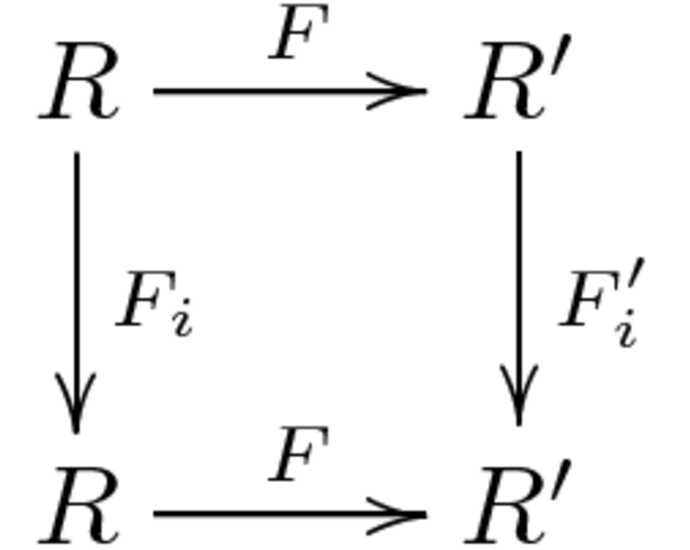
\includegraphics{master_master-12.png}}
  \end{center}
  commutes as well with vertical arrows being isomorphisms. This implies that
  if for $x \in R$ we have $F_i (x) = x$, then $F_i' (F (x)) = F (x)$, which
  implies the required claim.
  
  We next prove the second statement. Note first that the only added
  hypothesis is that $F$ induces an isomorphism between CAS. The fact that the
  diagram
  
  \begin{center}
    \resizebox{0.7\columnwidth}{!}{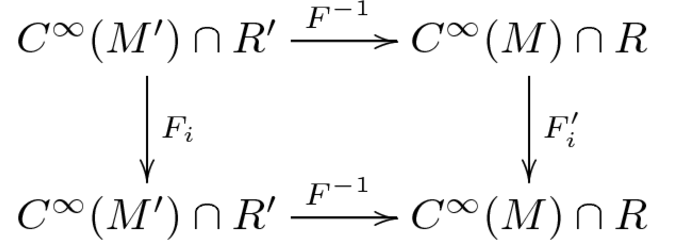
\includegraphics{master_master-13.png}}
  \end{center}
  
  commutes: it follows automatically (by simple computations). Now, the
  required statement follows by a symmetric argument.
\end{proof}

\begin{proof}
  (of prop. \ref{CAS:prop-restriction}) We take $\Gamma$ is given by lemma
  \ref{CAS:lem-aux}, and we only need to show that $\Gamma \cap N_{H \subset
  G} = \varnothing$ and that the distributional pullback gives the map of CAS
  $\mathcal{D}' (G)_P \rightarrow \mathcal{D}' (H)_{H_P}$. Now the former is
  true, as map $H \times P \ni (h, p) \mapsto h p \in G$ is onto, hence the
  dual of its derivative $T_{h p}^{\ast} G \rightarrow T_h^{\ast} H \oplus
  T_p^{\ast} P$ is injective at every point, so it remains only to prove the
  latter. It is also true, however, as lemma \ref{CAS:lem-aux} implies that
  convergence in $\mathcal{D}' (G)_P$ implies that in $\mathcal{D}'_{\Gamma}
  (G)$ and the sequential continuity of pullback then gives the desired.
\end{proof}

\begin{proof}
  (of prop. \ref{CAS:prop-proj}) The fact that both sides are CAS follows from
  the proposition \ref{CAS:prop-GoverP}. The fact that map $\mathcal{D}' (G)
  \mapsto \mathcal{D}' (G \times H)_H$ is is map of CAS is clear by continuity
  of $\otimes$, so we only need to prove that the inverse is well-defined map
  of CAS. Now, let $f_n \in \mathcal{D}' (G \times H)_H$ converging in
  $\mathcal{D}' (G \times H)$. We then have by fact \ref{fact:sing-q-4} that
  $f_n = \varphi_n \otimes \rho$ with $\varphi_n \in \mathcal{D}' (G)$ and
  definition of $\otimes$ then implies the convergence of $\varphi_n$.
\end{proof}

\section{Holomorphicity of symmetry breaking operators}\label{sec:holoop}

\subsection{Main results}

\begin{definition}
  \label{holoop:def-weakholo}Suppose $\Omega \subset \mathbbm{C}^m$ is an open
  domain and $\lambda (\cdot), \nu (\cdot)$ are holomorphic on $\Omega$.
  Suppose further that for every $\mu \in \Omega$ we have $H_{\mu} \in
  \tmop{Hom}_{G'} (I (\lambda (\mu)), J (\nu (\mu)))$.
  
  Now, for $K_M \assign M \cap K$ and $K_M' \assign P' \cap K_M$ the
  $K$-equivariant diffeomorphism $K / K_M \rightarrow G / P$ induces
  $K$-diffeomorphism between vector bundles $G \times_{\lambda} \mathbbm{C}$
  over $G / P$ and $\mathbbm{C} \times K / K_M$ over $K_M$. These induce \
  Frechet space isomorphisms $C^{\infty} (K / K_M) \simeq I (\lambda)$ and
  $C^{\infty} (K' / K_M') \simeq J (\nu)$ which are respectively $K$ and
  $K'$-equivariant. These induce the inclusion $\tmop{Hom}_{G'} (I (\lambda),
  J (\nu)) \hookrightarrow \tmop{Hom}_{K'} (C^{\infty} (K / K_M), C^{\infty}
  (K' / K_M'))$.
  
  We say that $H_{\mu}$ is \tmtextbf{weakly holomorphic in} $\mu \in \Omega$
  if for every $K$-finite $f \in C^{\infty} (K / K_M)_K$ and $K'$-finite $g
  \in C^{\infty} (K' / K_M')_{K'}$ we have $\langle H_{\mu} f, g \rangle$
  being holomorphic in $\mu$.
\end{definition}

\begin{remark}
  One can give similar definitions for $H_{\mu} \in \tmop{Hom}_G (I (\lambda
  (\mu)), I (\lambda' (\mu)))$ and we shall use them in what follows.
\end{remark}

\begin{proposition}
  \label{holoop:prop-comp-of-holo-is-holo}Suppose $\Omega \subset
  \mathbbm{C}^m$ open domain with $\lambda' (\cdot), \lambda (\cdot), \nu
  (\cdot), \nu' (\cdot)$ being all holomorphic on $\Omega$. Suppose further
  that $A_{\mu} \in \tmop{Hom}_G (I (\lambda' (\mu)), I (\lambda (\mu)))$,
  $B_{\mu} \in \tmop{Hom}_{G'} (I (\lambda (\mu)), J (\nu (\mu)))$ and
  $C_{\mu} \in \tmop{Hom}_{G'} (J (\nu (\mu)), J (\nu' (\mu)))$ are weakly
  holomorphic. Then, the compositions $B_{\mu} \circ A_{\mu}$ and $C_{\mu}
  \circ B_{\mu}$ are also so.
\end{proposition}

\begin{proposition}
  \label{holoop:prop-holo-rigidity}Suppose $A_{\mu} \in \tmop{Hom} (\lambda
  (\mu), \nu (\mu))$ is weakly holomorphic in $\mu \in \Omega$ and $A_{\mu} =
  0$ for $\mu \in \Omega' \subset \Omega$: open subset. Then $A_{\mu} = 0$ on
  $\Omega$ as well.
\end{proposition}

\begin{proposition}
  \label{holoop:prop-main}Suppose $\Omega \subset \mathbbm{C}^m$ is open set
  with $\lambda (\cdot), \nu (\cdot)$ holomorphic on it and $K_{\mu} \in
  \mathcal{S} \tmop{ol} (\mathbbm{R}^{p, q} ; \lambda (\mu), \nu (\mu))$ is
  holomorphic in $\mu \in \Omega$ distribution. Then the corresponding element
  $H_{\mu} \in \tmop{Hom}_{G'} (I (\lambda (\nu)), J (\nu (\nu)))$ is weakly
  holomorphic.
\end{proposition}

\begin{remark}
  Similar proposition (with similar proof that will be omitted) holds for
  $K_{\mu} \in \mathcal{S} \tmop{ol}_{(G, G)} (\mathbbm{R}^{p, q} ; \lambda
  (\mu), \lambda' (\mu))$ (see definition \ref{knappstein:def-sol}).
\end{remark}

\begin{proposition}
  \label{holoop:prop-sphermult}Let $H \in \tmop{Hom}_{G'} (I (\lambda), J
  (\nu))$ and $K \in \mathcal{S} \tmop{ol} (\mathbbm{R}^{p, q} ; \lambda,
  \nu)$ be the corresponding kernel. Proposition
  \ref{k-finite:prop-holo-to-holo} establishes the injective map of vector
  spaces $\mathcal{S} \tmop{ol} (\mathbbm{R}^{p, q} ; \lambda, \nu)
  \hookrightarrow \mathcal{D}' (\mathbbm{S}^p \times \mathbbm{S}^q)$ and we
  let $K^S \in \mathcal{D}' (\mathbbm{S}^p \times \mathbbm{S}^q)$ be the image
  of $K$. Let further (with reference to maps discussed in definition
  \ref{holoop:def-weakholo}) $1_{\lambda}$ and $1_{\nu}$ be spherical vectors
  defined as $C^{\infty} (\mathbbm{S}^p \times \mathbbm{S}^q) \ni 1 \mapsto
  1_{\lambda} \in I (\lambda)$ and $C^{\infty} (\mathbbm{S}^{p - 1} \times
  \mathbbm{S}^q) \ni 1 \mapsto 1_{\nu} \in J (\nu)$. Then $G'$-equivariance
  and the structure of $(\mathfrak{g}, K)$-modules $C^{\infty} (\mathbbm{S}^p
  \times \mathbbm{S}^q)_K, C^{\infty} (\mathbbm{S}^{p - 1} \times
  \mathbbm{S}^q)_{K'}$ imply that $H 1_{\lambda} = c 1_{\nu}$ for some $c \in
  \mathbbm{C}$.
  
  We have $c = \frac{1}{2} \langle K^S, 1 \rangle_{\mathbbm{S}^p \times
  \mathbbm{S}^q}$.
\end{proposition}

\subsection{Auxiliary lemmas}

\begin{definition}
  \label{holoop:def-strongholo}Let the setting be as in definition
  \ref{holoop:def-weakholo}. Now, for $K_M \assign M \cap K$ and $K_M' \assign
  P' \cap K_M$ the $K$-equivariant diffeomorphism $K / K_M \rightarrow G / P$
  induces $K$-morphism between vector bundles $G \times_{\lambda} \mathbbm{C}$
  over $G / P$ and $\mathbbm{C} \times K / K_M$ over $K_M$, thus its
  completion induces $\mathcal{D}' (G / P \times G' / P', \mathbbm{C}_{\lambda
  - n} \boxtimes \mathbbm{C}_{\nu})^{G'} \hookrightarrow \mathcal{D}' (K / K_M
  \times K' / K_M')^{K'}$ map.
  
  We say $H_{\mu}$ is \tmtextbf{strongly holomorphic in $\mu \in \Omega$} if
  the image of $H_{\mu}$ in $\mathcal{D}' (K / K_M \times K' / K_M')^{K'}$ is
  holomorphic.
\end{definition}

\begin{lemma}
  \label{holoop:lem-strong-implies-weak}Strong holomorphicity implies weak
  holomorphicity.
\end{lemma}

\begin{proof}
  Re-examining the definitions \ref{holoop:def-strongholo} and
  \ref{holoop:def-weakholo}, we note that the statement would be implied by
  the commutativity of the diagram
  
  \begin{center}
    \resizebox{0.7\columnwidth}{!}{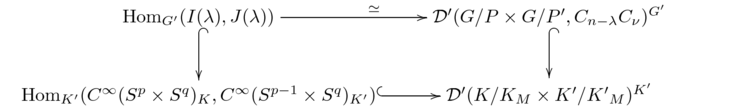
\includegraphics{master_master-14.png}}
  \end{center}
  
  where $\mathcal{D}' (K / K_M \times K' / K'_M)^{K'} \assign \left\{ f \in
  \mathcal{D}' (K / K_M \times K' / K'_M) \big| \forall k' \in K', \; f (k'
  \cdot, k' \cdot) = f (\cdot, \cdot) \right\}$ and with left and right arrows
  as in definitions \ref{holoop:def-weakholo} and \ref{holoop:def-strongholo}
  respectively and horizontal arrows implied by Schwartz theorem, as strong
  holomorphicity implies that corresponding element of $\mathcal{D}' (K / K_M
  \times K' / K'_M)^{K'}$ is holomorphically dependent on a parameter, hence
  for $(f, g) \in C^{\infty} (\mathbbm{S}^p \times \mathbbm{S}^q)_K \times
  C^{\infty} (\mathbbm{S}^{p - 1} \times \mathbbm{S}^q)_{K'}$ we have $\langle
  H f, g \rangle = \langle K, f \otimes g \rangle$ being holomorphic, where $H
  \in \tmop{Hom}_{G'} (I (\lambda), J (\nu))$ and $K \in \mathcal{D}' (K / K_M
  \times K' / K_M')^{K'}$ corresponding.
  
  We now explain why the diagram commutes. It follows by direct computations,
  as all arrows are induced by the same pullbacks of vector bundles: $G
  \times_P \mathbbm{C}_{n - \lambda}$ over $G / P$ pulled back to direct
  bundle over $K / K_M$ via the $K / K_M^{} \tilde{\rightarrow} G / P$ and $G'
  \times_{P'} \mathbbm{C}_{\nu}$ over $G' / P'$ pulled back to direct over $K'
  / K_M'$ via the $K' / K_M' \tilde{\rightarrow} G' / P'$.
\end{proof}

\begin{lemma}
  \label{holoop:lem-main}Holomorphicity of $K_{\mu} \in \mathcal{S} \tmop{ol}
  (\mathbbm{R}^{p, q} ; \lambda (\mu), \nu (\mu))$ implies strong
  holomorphicity.
\end{lemma}

\begin{proof}
  With maps as in digram in lemma \ref{holoop:lem-commdiag}, the
  holomorphicity of $K_{\mu} \in \mathcal{S} \tmop{ol} (\mathbbm{R}^{p, q} ;
  \lambda (\mu), \nu (\mu))$, implies the holomorphicity of corresponding
  $K_{\mu} \in \mathcal{D}'_{\lambda (\mu) - n} (\Xi)^{P'}$ (by lemma
  \ref{k-finite:prop-holo-to-holo}) and then by lemma
  \ref{holoop:lem-main-aux} the holomorphicity of corresponding $K_{\mu} \in
  \mathcal{D}' (G)_P^{P'}$ (we allow ourselves small abuse of notation, using
  $K_{\mu}$ to denote several things).
  
  We next observe that map $\mathcal{D}' (G \times G')_{P \times P'}^{G'}$
  exhibited in lemma \ref{holoop:lem-commdiag} is seen to be defined as
  restriction of the map $\mathcal{D}' (G \times G')_{P \times 1}^{G'}
  \rightarrow \mathcal{D}' (G \times G')_{P \times 1}^{R (G')}$ exhibited in
  lemma \ref{holoop:lem-main-commdiag}, and the commutativity of the diagram
  in the latter lemma implies that the corresponding element $\mathcal{D}'
  (K)_{K_M}$ is holomorphic due to proposition
  \ref{holomorphicity-preserving:prop-pullback-holo}.
\end{proof}

\begin{lemma}
  \label{holoop:lem-main-commdiag}The following diagram of vector spaces
  commutes:
  
  \begin{center}
    \resizebox{0.7\columnwidth}{!}{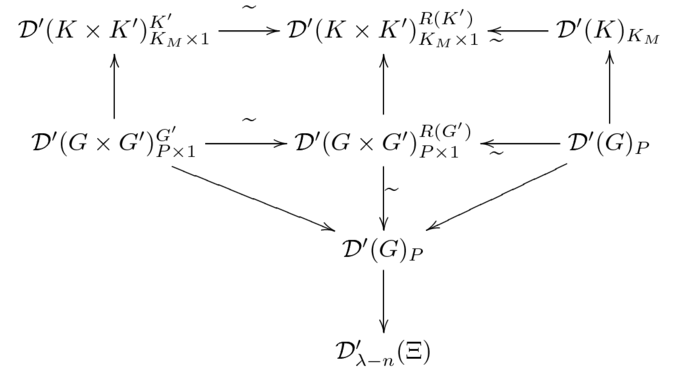
\includegraphics{master_master-15.png}}
  \end{center}
  
  Here the spaces are as follows:
  \begin{enumerate}
    \item $\mathcal{D}' (G \times G')_{P \times 1}^{R (G')} \assign \{ f \in
    \mathcal{D}' (G \times G') | \forall (g', p) \in G' \times P, e^{\nu^{- 1}
    (g')} f (\cdot, \cdot g') = e^{(\lambda - n) (p)} f (p \cdot, \cdot) = f
    (\cdot, \cdot) \}$ and $\mathcal{D}' (K \times K')_{K_M \times 1}^{R
    (K')}$ similarly;
    
    \item all others are as in lemma \ref{holoop:lem-commdiag},
  \end{enumerate}
  and the maps are as follows:
  \begin{enumerate}
    \item three upmost vertical maps are as follows:
    \begin{enumerate}
      \item the leftmost is as in lemma \ref{holoop:lem-commdiag-aux1};
      
      \item the middle one is defined so to make rightmost square commute;
      
      \item the rightmost is given by proposition \ref{CAS:prop-restriction};
    \end{enumerate}
    \item The map $\mathcal{D}' (G \nobracket \times G' \nobracket)^{R
    (G')}_{P \times 1} \rightarrow \mathcal{D}' (G)_P$ is defined with the use
    of proposition \ref{CAS:prop-proj} (which gives $\mathcal{D}' (G \times
    G')^{R (G')} \rightarrow \mathcal{D}' (G)$ map) and proposition
    \ref{CAS:prop-invariant};
    
    \item the map $\mathcal{D}' (G \nobracket \times G' \nobracket)^{R
    (G')}_{P \times 1} \rightarrow \mathcal{D}' (G)_P$ is inverse of map in
    previous item;
    
    \item The map $\mathcal{D}' (G)_P \rightarrow \mathcal{D}' (G)_P$ is just
    identity map;
    
    \item The map $\mathcal{D}' (G)_P \rightarrow \mathcal{D}'_{\lambda - n}
    (\Xi)$ is as in lemma \ref{holoop:lem-commdiag};
    
    \item The map $\mathcal{D}' (G \times G')_{P \times 1}^{G'} \rightarrow
    \mathcal{D}' (G)_P$ is defined so to make the triangle commute
  \end{enumerate}
\end{lemma}

\begin{proof}
  The commutativity of left triangle is clear from the statement. The
  commutativity of right triangle is also so by the way we defined maps. The
  rightmost square commutes by definition. We note that this implies that
  $\mathcal{D}' (G \times G')_{P \times 1}^{R (G')} \rightarrow \mathcal{D}'
  (K \times K')^{R (K')}_{K_M \times 1}$ is in fact map of CAS (as
  $\mathcal{D}'  (G)_P \rightarrow \mathcal{D}' (K)_{K_M}$ is so by
  proposition \ref{CAS:prop-restriction}).
  
  Finally, the leftmost square commutes as it is map of CAS and commutes when
  we start from smooth elements.
\end{proof}

\begin{lemma}
  \label{holoop:lem-main-aux}Let the map $\mathcal{D}' (G)_P
  \tilde{\rightarrow} \mathcal{D}'_{\lambda} (\Xi)$ be as given by proposition
  \ref{CAS:prop-GoverP}. Suppose further that $\lambda = \lambda (\mu)$ is the
  value of holomorphic function function defined on $\Omega \subset
  \mathbbm{C}^{\mu}$ open and $f_{\mu} \in \mathcal{D}' (\Xi)$ is holomorphic
  such that $f_{\mu} \in \mathcal{D}'_{\lambda (\mu)} (\Xi)$. Then the
  preimage under $\mathcal{D}' (G)_P \tilde{\rightarrow}
  \mathcal{D}'_{\lambda} (\Xi)$, which we call $F_{\mu} \in \mathcal{D}'
  (G)_P$ is holomorphic in $\mathcal{D}'_{\Gamma} (G)$, where $\Gamma$ is as
  defined in lemma \ref{CAS:lem-aux}.
\end{lemma}

\begin{proof}
  First, the holomorphicity of $F_{\mu}$ is readily implied by proposition
  \ref{CAS:prop-GoverP-holo}. Next, we let $\mathfrak{a}$ be some complement
  of $\mathfrak{p} \assign \tmop{Lie} (P)$ in $\mathfrak{g}$, so that
  $\mathfrak{g}=\mathfrak{p} \oplus \mathfrak{a}$ and $\mathfrak{g}^{\ast}
  =\mathfrak{p}^{\ast} +\mathfrak{a}^{\ast}$. It then suffices to prove the
  desired statement locally, so we take arbitrary $g_0 \in G$ and as the map
  $\mathfrak{a} \times P \ni (X, p) \mapsto g_0 \exp (X) p \in G$ is local
  diffeomorphism near $g_0$, we have small neighborhood $U \ni g_0$ being
  diffeomorphic to $\mathfrak{a} \times P \supset V \times O \ni (0, 1)$
  neighborhood. When pulling back to $V \times O$ the $F_{\mu} \big|_U$ and
  applying fact \ref{fact:sing-q-4}, we see that the image is of the form
  $\psi_{\mu} \otimes e^{\lambda (\mu) (\cdot)} \in \mathcal{D}' (V) \otimes
  C^{\infty} (O)$ and as $F_{\mu} \big|_U$ and $\lambda (\cdot)$ were
  holomorphic, so will be $\psi_{\mu} \in \mathcal{D}' (V)$ (we recall that
  $e^{\lambda (\mu) (\cdot)} \neq 0$). Hence, in the light of proposition
  \ref{holomorphicity-preserving:prop-tensor-holo}, we only need to show that
  $e^{\lambda (\mu) (\cdot)}$ is holomorphic in $\mathcal{D}'_{\varnothing}
  (O)$. Now, pulling back via $\exp : \mathfrak{p} \rightarrow P$ which is
  diffeomorphism near $0 \ni \mathfrak{p}$, we see that it suffices to prove
  the following:
  
  {\noindent}\tmtextbf{Claim . }\tmtextit{Suppose that $\lambda : \Omega
  \rightarrow \mathbbm{C}^n$ is vector-valued analytic function. Then, when
  seen as parametrized distribution on $\mathbbm{R}^n$ via $x \mapsto \langle
  \lambda (\cdot), x \rangle$ it is holomorphic in $\mathcal{D}'_{\varnothing}
  (\mathbbm{R}^n)$.}{\hspace*{\fill}}{\medskip}
  
  Indeed, recalling the defintion
  \ref{holomorphicity-preserving:def-holo-in-DG} and that in {\cite[def.
  8.2.2]{hormander1983analysis}}, we see that it suffices to show that as
  $\Omega \ni \mu_j \rightarrow \mu_0 \in \Omega$, we have for $u_j \in
  \langle \lambda (\mu_j), \cdot \rangle \in \mathcal{D}'_{\varnothing}
  (\mathbbm{R}^n)$ and arbitrary $\psi \in C^{\infty}_0 (\mathbbm{R}^n)$ and
  arbitrary $N$,
  \[ \sup_j \quad \sup_{\xi \in \mathbbm{R}^n} | \xi |^N | \widehat{\psi u_j}
     (\xi) | < \infty . \]
  Now, {\cite[lemma 7.1.3]{hormander1983analysis}} implies that for this it
  suffices to show that for arbitrary $\alpha, \beta \in
  \mathbbm{Z}^n_{\geqslant 0}$ we have
  \[ \sup_{\xi \in \mathbbm{R}^n} | D_{\beta} (x^{\alpha} \psi u_j) | <
     \infty, \]
  and as the latter is clear, we are done.
\end{proof}

\begin{lemma}
  \label{holoop:lem-sphermult-aux}Let $K$, $H$ and $K^S$ be as in proposition
  \ref{holoop:prop-sphermult}. As in definition \ref{holoop:def-strongholo} we
  have corresponding to $H$ an element $H^S \in \mathcal{D}' (K / K_M \times
  K' / K_M')^{K'}$. We then consider a map
  \[ T : \mathcal{D}' (K / K_M \times K' / K_M')^{K'} \tilde{\rightarrow}
     \mathcal{D}' (K \times K')_{K_M \times K_M'}^{K'} \tilde{\rightarrow}
     \mathcal{D}' (K \times K')_{K_M \times K_M'}^{R (K')} \tilde{\rightarrow}
     \mathcal{D}' (K)^{K'_M}_{K_M} \tilde{\rightarrow} \mathcal{D}' (K /
     K_M)^{K'_M}, \]
  where the maps from left to right are respectively:
  \begin{enumerate}
    \item Completion of the obvious map $C^{\infty} (K / K_M \times K' / K_M')
    \rightarrow C^{\infty} (K \times K')_{K_M \times K_M'}$ where
    \[ C^{\infty} (K \times K')_{K_M \times K_M'} \assign \left\{ f \in
       C^{\infty} (K \times K') \big| \forall (k, k') \in K \times K', \; f
       (\cdot k, \cdot k') = f (\cdot, \cdot) \right\} \]
    and similarly $\mathcal{D}' (K \times K')_{K_M \times K_M'}$ is defined;
    
    \item Induced by diffeomorphism $K \times K' \ni (k, k') \mapsto ((k')^{-
    1} k, k') \in K \times K'$, where
    \[ \mathcal{D}' (K \times K')_{K_M \times K_M'}^{R (K')} \assign \left\{
       f \in \mathcal{D}' (K \times K')_{} \big| \forall (k, k', k'') \in
       K_M \times K_M' \times K', \; f ((k')^{- 1} \cdot k, k'' \cdot k') = f
       (\cdot, \cdot) \right\} ; \]
    \item Restriction onto the first coordinate (makes sense by the
    $K'$-invariance of elements of $\mathcal{D}' (K \times K')^{R (K')}_{K_M
    \times K_M'}$), where we let $\mathcal{D}' (K)^{K'_M}_{K_M} \assign
    \left\{ f \in \mathcal{D}' (K) \big| \forall (k, k') \in K_M' \times
    K', \; f (k \cdot k') = f (\cdot) \right\}$;
    
    \item Induced by $\mathcal{D}' (K)_{K_M} \rightarrow \mathcal{D}' (K /
    K_M)$ map (see proposition \ref{CAS:prop-GoverP} and apply proposition
    \ref{CAS:prop-invariant} with $\{ C^{\infty} (K)_{K_M} \ni f (\cdot)
    \mapsto f (k \cdot) \in C^{\infty} (K)_{K_M} \}_{k \in K'}$ and $\{
    C^{\infty} (K / K_M)_{} \ni f (\cdot) \mapsto f (k \cdot) \in C^{\infty}
    (K / K_M)_{} \}_{k \in K'}$)
  \end{enumerate}
  We then have $T H^S = K^S$ (where we identify space of even members of
  $\mathcal{D}' (\mathbbm{S}^p \times \mathbbm{S}^q)$ with $\mathcal{D}' (K /
  K_M)$ by the diffeomorphism $K / K_M \simeq \mathbbm{S}^p \times
  \mathbbm{S}^q / \{ \pm \}$). Moreover, $T$ is an isomorphism of CAS.
\end{lemma}

\begin{proof}
  The first part is a direct implication of lemma \ref{holoop:lem-commdiag}.
  We now show that $T$ is an isomorphism of CAS. As $T$ is continuous, is
  isomorphism and maps $C^{\infty} (K / K_M \times K' / K_M')^{K'}$ onto
  $C^{\infty} (K / K_M)^{K'_M}$, it suffices to show that both spaces are CAS.
  We start with $\mathcal{D}' (K / K_M')^{K_M'}$. It is clear that if
  $C^{\infty} (K / K_M)^{K_M'} \ni f_n \rightarrow f \in \mathcal{D}' (K /
  K_M)$, then $f \in \mathcal{D}' (K / K_M)^{K_M'}$. Moreover, if $f \in
  \mathcal{D}' (K / K_M)^{K_M'}$ and we take $C^{\infty} (K / K_M) \ni f_n
  \rightarrow f$, we can let $f_n' (\cdot) = \int_{k \in K_M'} f_n (k \cdot) d
  k$ and then $f_n' \in C^{\infty} (K / K_M')^{K_M'}$, while still $f_n'
  \rightarrow f$. This shows that $\mathcal{D}' (K / K_M')^{K_M'}$ is CAS. The
  fact that $\mathcal{D}' (K / K_M \times K' / K_M')^{K'}$ is CAS now follows
  from continuity of $T$.
\end{proof}

\begin{lemma}
  \label{holoop:lem-commdiag}The following diagram of maps between vector
  spaces commutes:
  
  \begin{center}
    \resizebox{0.7\columnwidth}{!}{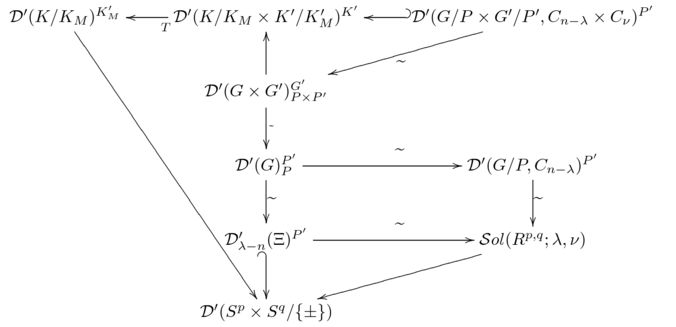
\includegraphics{master_master-16.png}}
  \end{center}
  
  The spaces are defined as follows:
  \begin{eqnarray}
    & \mathcal{D}' (G \times G')_{P \times P'}^{P'} \assign \{ f \in
    \mathcal{D}' (G \times G') | \forall (p, p') \in P \times P', f (p' \cdot,
    p' \cdot) = e^{- \nu (p')} e^{- (\lambda - n) (p)} f (\cdot p, \cdot p') =
    f (\cdot, \cdot) \} &  \nonumber\\
    & \mathcal{D}' (G)_P^{P'} \assign \left\{ f \in \mathcal{D}' (G) \big|
    \forall (p, p') \in P \times P', \; e^{\nu (p')} f (p' \cdot) = e^{-
    (\lambda - n) (p)} f (\cdot p) = f (\cdot) \right\} &  \nonumber
  \end{eqnarray}
  And the maps are as:
  \begin{enumerate}
    \item the map $\mathcal{D}' (G / P \times G' / P', \mathbbm{C}_{n -
    \lambda} \times \mathbbm{C}_{\nu}) \rightarrow \mathcal{D}' (K / K' \times
    K' / K_M')$ is induced by diffeomorphism $K / K_M \rightarrow G / P$ (and
    same for primes) which induces $K$-morphism from $\mathbbm{C}_{n -
    \lambda}$ over $G / P$ to trivial bundle over $K / K_M$;
    
    \item $\mathcal{D}' (G / P \times G' / P', \mathbbm{C}_{n - \lambda}
    \times \mathbbm{C}_{\nu})^{P'} \rightarrow \mathcal{D}' (G \times
    G')^{P'}_{P \times P'}$ is induced by isomorphism $\mathcal{D}' (G / P
    \times G' / P', \mathbbm{C}_{n - \lambda} \times \mathbbm{C}_{\nu})
    \rightarrow \mathcal{D}' (G \times G')_{P \times P'}^{P'}$ of CAS (by
    proposition \ref{CAS:prop-GoverP}) via prop. \ref{CAS:prop-invariant};
    
    \item $\mathcal{D}' (G \times G')_{P \times P'}^{P'} \rightarrow
    \mathcal{D}' (K / K_M \times K' / K_M')^{K'}$ is composition
    \[ \mathcal{D}' (G \times G')_{P \times P'}^{P'} \rightarrow \mathcal{D}'
       (K \times K')_{K_M \times K_M'}^{K'} \rightarrow \mathcal{D}' (K / K_M
       \times K' / K_M')^{K'} \]
    where last morphism is by propositions \ref{CAS:prop-GoverP} and
    \ref{CAS:prop-invariant}, while the first one is given by propositions
    \ref{CAS:prop-restriction} (which gives $\mathcal{D}' (G \times G')_{P
    \times P'} \rightarrow \mathcal{D}' (K \times K')_{K_M \times K_M'}$
    CAS-map) and \ref{CAS:prop-invariant};
    
    \item $\mathcal{D}' (G \times G')^{G'}_{P \times P'} \rightarrow
    \mathcal{D}' (G)_P^{P'}$ is induced via prop. \ref{CAS:prop-invariant} via
    isomorphism
    \begin{eqnarray}
      & \mathcal{D}' (G \times G')^{G'} \assign \left\{ f \in \mathcal{D}' (G
      \times G') \big| \forall p' \in G', \; f (p' \cdot, p' \cdot) = f
      (\cdot, \cdot) \right\} \rightarrow \mathcal{D}' (G) &  \nonumber
    \end{eqnarray}
    of CAS, which is defined as composistion of pullback by diffeomorphism $G
    \times G' \ni (g, g') \mapsto ((g')^{- 1} g, g') \in G \times G'$ and
    application of prop. \ref{CAS:prop-proj};
    
    \item $\mathcal{D}' (G)_P^{P'} \rightarrow \mathcal{D}' (G / P,
    \mathbbm{C}_{n - \lambda})^{P'}$ is by proposition \ref{CAS:prop-GoverP}
    (granting $\mathcal{D}' (G)_P \rightarrow \mathcal{D}' (G / P,
    \mathbbm{C}_{n - \lambda})$ isomorphism of CAS) and proposition
    \ref{CAS:prop-invariant};
    
    \item $\mathcal{D}' (G)_P^{P'} \rightarrow \mathcal{D}'_{\lambda - n}
    (\Xi)^P$ is by proposition \ref{CAS:prop-GoverP} (granting $\mathcal{D}'
    (G)_{M_0 N_+} \rightarrow \mathcal{D}' (\Xi)$ isomorphism of CAS, note
    that $G \curvearrowright \Xi$ has $M_0 N_+$ as stabilizer of $(1, 0_{p +
    q}, 1)$ with $M_0 \subset M$ of index 2) and proposition
    \ref{CAS:prop-invariant};
    
    \item $\mathcal{D}' (G / P, \mathbbm{C}_{n - \lambda})^{P'} \rightarrow
    \mathcal{S} \tmop{ol} (\mathbbm{R}^{p, q} ; \lambda, \nu)$ is a pullback
    via embedding $\mathbbm{R}^{p, q} \simeq \mathfrak{n}_+
    \longhookrightarrow G / P$ (note that we can trivialize $\mathbbm{C}_{n -
    \lambda}$ above $\mathfrak{n}_+$);
    
    \item $\mathcal{D}'_{\lambda - n} (\Xi)^{P'} \rightarrow \mathcal{S}
    \tmop{ol} (\mathbbm{R}^{p, q} ; \lambda, \nu)$ is pullback via embedding
    $\mathbbm{R}^{p, q} \longhookrightarrow \Xi$ as in proposition
    \ref{k-finite:prop-claim2} (it also shows that it's an isomorphism);
    
    \item $\mathcal{D}'_{\lambda - n} (\Xi)^{P'} \rightarrow \mathcal{D}' 
    (\mathbbm{S}^p \times \mathbbm{S}^q / \{ \pm \})$ is pullback via
    embedding $\mathbbm{S}^p \times \mathbbm{S}^q \longhookrightarrow \Xi$;
    
    \item map $\mathcal{S} \tmop{ol} (\mathbbm{R}^{p, q} ; \lambda, \nu)
    \rightarrow \mathcal{D}' (\mathbbm{S}^p \times \mathbbm{S}^q)$ is the
    composition of inverse of $\mathcal{D}'_{\lambda - n} (\Xi)^{P'}
    \rightarrow \mathcal{S} \tmop{ol} (\mathbbm{R}^{p, q} ; \lambda, \nu)$
    isomorphism (see prop. \ref{k-finite:prop-claim2}) and pullback via
    $\mathbbm{S}^p \times \mathbbm{S}^q \longhookrightarrow \Xi$ (we note that
    it's easy to observe that $\{ f \in \mathcal{D}' (\mathbbm{S}^p \times
    \mathbbm{S}^q) | f (- \cdot, - \cdot) = f (\cdot, \cdot) \} \rightarrow
    \mathcal{D}' (\mathbbm{S}^p \times \mathbbm{S}^q / \{ \pm \})$ is
    isomorphism of CAS).
  \end{enumerate}
\end{lemma}

\begin{proof}
  We first note that the triangle involving $\mathcal{D}'_{\lambda - n}
  (\Xi)^{P'}$, $\mathcal{S} \tmop{ol} (\mathbbm{R}^{p, q} ; \lambda, \nu)$ and
  $\mathcal{D}' (\mathbbm{S}^p \times \mathbbm{S}^q / \{ \pm \})$ commutes by
  definition of $\mathcal{S} \tmop{ol} (\mathbbm{R}^{p, q} ; \lambda, \nu)
  \rightarrow \mathcal{D}' (\mathbbm{S}^p \times \mathbbm{S}^q / \{ \pm \})$
  map.
  
  Next, we claim that the rectangle involving $\mathcal{D}'_{\lambda - n}
  (\Xi)^{P'}$, $\mathcal{D}' (G)_P^{P'}$, $\mathcal{S} \tmop{ol}
  (\mathbbm{R}^{p, q} ; \lambda, \nu)$ and $\mathcal{D}' (G / P,
  \mathbbm{C}_{n - \lambda})^{P'}$ commutes. Indeed, if we leave arrows intact
  and replace vertices by respectively $\mathcal{D}'_{\lambda - n} (\Xi)$,
  $\mathcal{D}' (G)_P$, $\mathcal{D}' (\mathbbm{R}^{p, q})$ and $\mathcal{D}'
  (G / P, \mathbbm{C}_{n - \lambda})$ respectively, the obtained diagram will
  be the diagram of CAS (by proposition \ref{CAS:prop-GoverP} applied to upper
  and left arrows and properties of distribution pullback; note that
  $\mathcal{D}'_{\lambda - n} (\Xi) \rightarrow \mathcal{D}' (\mathbbm{S}^p
  \times \mathbbm{S}^q / \{ \pm \}) \tmop{and} \mathcal{D}'_{\lambda - n}
  (\Xi) \rightarrow \mathcal{D}' (\mathbbm{R}^{p, q})$ are maps of CAS) which
  has then to commute, as it does so if we start from the member of
  $\mathcal{D}' (G)_P$. Hence, the original rectangle formed a commuting
  diagram.
  
  Next, we claim that the triangle constisting of $\mathcal{D}' (K / K_M
  \times K' / K_M')^{K'}$, $\mathcal{D}' (G / P \times G' / P', \mathbbm{C}_{n
  - \lambda} \times \mathbbm{C}_{\nu})^{G'}$ and $\mathcal{D}' (G \times
  G')_{P \times P'}^{P'}$ commutes. We note that if we leave arrows the same
  and replace vertices by respectively $\mathcal{D}' (K / K_M \times K' /
  K_M')$, $\mathcal{D}' (G / P \times G' / P', \mathbbm{C}_{n - \lambda}
  \nobracket \times \mathbbm{C}_{\nu} \nobracket)$ and $\mathcal{D}' (G
  \nobracket \times G' \nobracket)_{P \times P'}$, then we obtain the diagram
  of CAS: indeed,
  \begin{enumerate}
    \item arrow $\mathcal{D}' (G / P \times G' / P', \mathbbm{C}_{n - \lambda}
    \times \mathbbm{C}_{\nu})_{} \rightarrow \mathcal{D}' (K / K_M \times K' /
    K_M')$ is induced by the fact that the direct bundle over $K / K_M \times
    K' / K_M'$ is pullback of $\mathbbm{C}_{n - \lambda} \times
    \mathbbm{C}_{\nu}$ over $G / P \times G' / P'$ and thus $\mathcal{D}' (G /
    P \times G' / P', \mathbbm{C}_{n - \lambda} \times \mathbbm{C}_{\nu})_{}
    \rightarrow \mathcal{D}' (K / K_M \times K' / K_M')$ is induced by
    pullback of smooth sections, hence is map of CAS;
    
    \item arrow $\mathcal{D}' (G / P \times G' / P', \mathbbm{C}_{n - \lambda}
    \nobracket \times \mathbbm{C}_{\nu} \nobracket) \rightarrow \mathcal{D}'
    (G \nobracket \times G' \nobracket)_{P \times P'}$ is isomorphism of CAS
    by proposition \ref{CAS:prop-GoverP};
    
    \item arrow $\mathcal{D}' (G \nobracket \times G' \nobracket)_{P \times
    P'} \rightarrow \mathcal{D}' (K / K_M \times K' / K_M')$ is a composition
    of $\mathcal{D}' (G \times G')_{P \times P'} \rightarrow \mathcal{D}' (K
    \times K')_{K_M \times K_M'}$ (given by proposition
    \ref{CAS:prop-restriction}) and $\mathcal{D}' (K \times K')_{K_M \times
    K_M'} \rightarrow \mathcal{D}' (K / K_M \times K' / K_M')$ given by prop.
    \ref{CAS:prop-GoverP}.
  \end{enumerate}
  The fact that the latter diagram of CAS commutes now follows, as it does so
  for smooth elements. Hence, the original diagram also commuted.
  
  Finally, we are to show that the triangle involving $\mathcal{D}' (K /
  K_M)^{K'_M}$, $\mathcal{D}' (\mathbbm{S}^p \times \mathbbm{S}^q / \{ \pm
  \})$ and $\mathcal{D}' (K / K_M \times K' / K_M')^{K'}$ commutes. We note
  that lemma \ref{holoop:lem-commdiag-aux1} implies that $\mathcal{D}' (G
  \times G')_{P \times P'}^{G'} \rightarrow \mathcal{D}' (K \times K')_{K_M
  \times K_{M'}}^{K'}$ can be seen as induced by map $\mathcal{D}' (G \times
  G')^{G'}_P \rightarrow \mathcal{D}' (K \times K')_{K_M}^{K'}$ of CAS as in
  the latter lemma. Thus, using proposition \ref{CAS:prop-invariant} we see
  that it suffices to show that the following diagram commutes:
  \begin{center}
    \resizebox{0.7\columnwidth}{!}{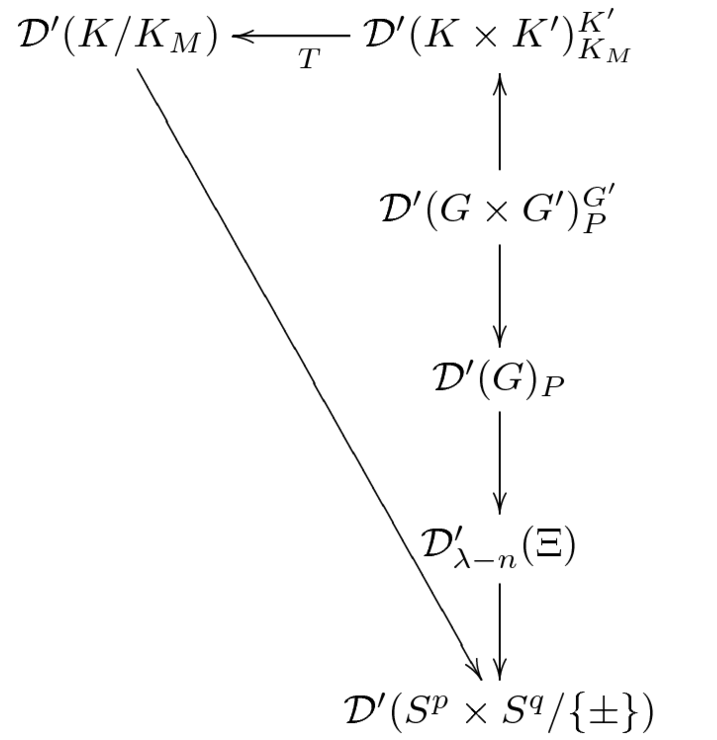
\includegraphics{master_master-17.png}}
  \end{center}
  We also note that every map of this diagram is the map of CAS by proposition
  \ref{CAS:prop-GoverP}, and hence it suffices to check that diagram commutes
  if we start from the element of $C^{\infty} (G \times G')^{G'}_P$. As the
  latter is verified directly to be true, we are done.
\end{proof}

\begin{lemma}
  \label{holoop:lem-commdiag-aux1}Let the setting be as in lemma
  \ref{holoop:lem-commdiag} and $T : \mathcal{D}' (G \times G')_{P \times P'}
  \rightarrow \mathcal{D}' (K \times K')_{K_M \times K_M'}$ be map of CAS
  given by proposition \ref{CAS:prop-restriction}. We then have the pullback
  map
  \begin{eqnarray}
    & C^{\infty} (G \times G')^{G'}_P \assign \left\{ f \in C^{\infty} (G
    \times G') \big| \forall (g', p) \in G' \times P, \; f (g' \cdot, g'
    \cdot) = f (\cdot p, \cdot) = f (\cdot, \cdot) \right\} \rightarrow & 
    \nonumber\\
    & \rightarrow C^{\infty} (K \times K')_{K_M}^{K'} \assign \left\{ f \in
    C^{\infty} (K \times K') \big| \forall (g', p) \in K' \times K_M, \; f
    (g' \cdot, g' \cdot) = f (\cdot p, \cdot) = f (\cdot, \cdot) \right\} & 
    \nonumber
  \end{eqnarray}
  induced by $K \times K' \longhookrightarrow G \times G'$, inducing map
  $\mathcal{D}' (G \times G')^{G'}_P \rightarrow \mathcal{D}' (K \times
  K')_{K_M}^{K'}$ of CAS which coincides with $T$ when restricted to
  $\mathcal{D}' (G \times G')_{P \times P'}^{G'}$.
\end{lemma}

\begin{proof}
  Lemma \ref{holoop:lem-aux} implies that the distributional pullback
  $\mathcal{D}' (G \times G')^{G'}_P \rightarrow \mathcal{D}' (K \times K')$
  is well-defined and the second item of lemma \ref{holoop:lem-aux} together
  with the fact that $\mathcal{D}' (G \times G')^{G'}_P$ is CAS implies that
  in fact the distributional pullback is a $\mathcal{D}' (G \times G')^{G'}_P
  \rightarrow \mathcal{D}' (K \times K')_{K_M}^{K'}$ map. Moreover, the second
  item implies that $\mathcal{D}' (G \times G')_P^{G'} \rightarrow
  \mathcal{D}' (K \times K')_{K_M}^{K'}$ is in fact map between CAS (that is,
  it is sequentially continuous) induced by pullback via $K \times K'
  \longhookrightarrow G \times G'$. Finally, proposition
  \ref{CAS:prop-restriction} implies that $T$ is the restriction of pullback
  of distributions $\mathcal{D}'_{\Gamma} (G \times G') \rightarrow
  \mathcal{D}' (K \times K')$ for some $\Gamma'$, while $\mathcal{D}' (G
  \times G')^{G'}_P \rightarrow \mathcal{D}' (K \times K')_{K_M}^{K'}$ is the
  restriction of $\mathcal{D}'_{\Gamma'} (G \times G') \rightarrow
  \mathcal{D}' (K \times K')$ pullback. Now, the fact that $C^{\infty} (G
  \times G')$ are dense in both $\mathcal{D}'_{\Gamma'} (G \times G'),
  \mathcal{D}'_{\Gamma} (G \times G')$ implies that they coincide when
  restricted to $\mathcal{D}' (G \times G')_{P \times P'}^{G'} \subset
  \mathcal{D}'_{\Gamma \cap \Gamma'} (G \times G')$.
\end{proof}

\begin{lemma}
  \label{holoop:lem-aux}Let the setting be as in lemma
  \ref{holoop:lem-commdiag}. Then,
  \begin{enumerate}
    \item there exists closed cone $\Gamma'$ such that $N_{K \times K' \subset
    G \times G'} \cap \Gamma' = \varnothing$ and $\mathcal{D}' (G \times
    G')_P^{G'} \subset \mathcal{D}'_{\Gamma'} (G \times G')$;
    
    \item Moreover, if $\varphi_n \in C^{\infty} (G \times G')_P^{G'}$
    converges in $\mathcal{D}' (G \times G')$, it converges in
    $\mathcal{D}'_{\Gamma'} (G \times G')$;
    
    \item both $\mathcal{D}' (G \times G')^{G'}_P, \mathcal{D}' (K \times
    K')_{K_M}^{K'}$ are CAS.
  \end{enumerate}
\end{lemma}

\begin{remark}
  Note that both normal bundle $N_{K \times K' \subset G \times G'}$ and
  $\Gamma'$ live in cotangent bundle $T^{\ast} (G \times G')$.
\end{remark}

\begin{proof}
  As the pullback by diffeomorphism $G \times G' \ni (g, g') \mapsto ((g')^{-
  1} g, (g')^{- 1}) \in G \times G'$ maps CAS to CAS (and similarly for $K
  \times K'$) and leaves $K \times K'$ invariant, it suffices to show the
  statements for
  \begin{eqnarray}
    & C^{\infty} (G \times G')^{R (G')}_P \assign \left\{ f \in C^{\infty} (G
    \times G') \big| \forall (g', p) \in G' \times P, \; f (\cdot, \cdot
    g') = f (\cdot p, \cdot) = f (\cdot, \cdot) \right\} &  \nonumber\\
    & C^{\infty} (K \times K')_{K_M}^{R (K')} \assign \left\{ f \in
    C^{\infty} (K \times K') \big| \forall (g', p) \in K' \times K_M, \; f
    (\cdot, \cdot g') = f (\cdot p, \cdot) = f (\cdot, \cdot) \right\} & 
    \nonumber
  \end{eqnarray}
  in place of $C^{\infty} (G \times G')^{G'}_P$ and $C^{\infty} (K \times
  K')_{K_M}^{K'}$ respectively. Proposition \ref{CAS:prop-GoverP} now readily
  implies the third item.
  
  Moreover, for every $(x_0, y_0) \in G \times G'$ we let $V_{(x_0, y_0)}
  \subset T_{(x_0, y_0)} G \times G'$ be the fiber at $(x_0, y_0)$ of the
  normal bundle of $G' \times P$ embedded in $G \times G'$ via $G' \times P
  \ni (g', p) \mapsto (x_0 p, y_0 g') \in G \times G'$. The set $\{ (x_0, y_0,
  V_{(x_0, y_0)}) | (x_0, y_0) \in G \times G' \}$ now forms a closed cone
  which we call $\Gamma'$ and lemma \ref{CAS:lem-aux} implies that
  $\mathcal{D}' (G \times G')_P^{G'} \subset \mathcal{D}'_{\Gamma'} (G \times
  G')$. Thus to prove the first item it suffices to show that at point $k_0
  \in K$ we have $N \cap N_{K \subset G} = \varnothing$, where $N$ denotes
  normal bundle of $P \ni p \mapsto k_0 p \in G$ submanifold. However, the
  latter follows, as $K \times P \ni (k, p) \mapsto k p \in G$ is onto, hence
  the dual of its derivative $T_{k_0}^{\ast} G \rightarrow T_{k_0}^{\ast}
  \oplus T_1^{\ast} P$ is in particular injective. This proves the first item.
  
  Finally, we the second item is readily implied by lemma \ref{CAS:lem-aux}.
\end{proof}

\subsection{Proofs}

\begin{proof}
  (of proposition \ref{holoop:prop-comp-of-holo-is-holo}) We first prove the
  weak holomorphicity of $B_{\mu} \circ C_{\mu}$. Indeed, we take $K$-finite
  vector $f \in C^{\infty} (K / K_M)_K$. As $\tmop{span} (K' f)$ is
  finite-dimensional, hence splits in finite number of $K'$-types, seeing
  $B_{\mu}$ as an element of $\tmop{Hom}_{K'} (C^{\infty} (K / K_M)_K,
  C^{\infty} (K' / K_M')_{K'})$, we see that $B_{\mu} f$ should lie in
  $\bigoplus_{\gamma \in \Gamma} C^{\infty} (K' / K_M') (\gamma)$ for some
  finite $\Gamma \subset \hat{K}'$ independent of $\mu$. Thus, admissibility
  of $(\mathfrak{g}', K')$-module $C^{\infty} (K' / K_M')_{K'}$ and the weak
  holomorphicity of $B_{\mu}$ imply that $B_{\mu} f = \sum_{i \in I} c_i (\mu)
  f_i$ for $I$ some finite set and $c_i (\mu)$ holomorphic. This ends the
  proof of this part, as $\langle C_{\mu} \circ B_{\mu} f, g \rangle = \sum_{i
  \in I} c_i (\mu) \langle C_{\mu} f_i, g \rangle$ is holomorphic in $\mu \in
  \Omega$.
  
  Next, we show that $B_{\mu} \circ A_{\mu}$ is weakly holomorphic. Similarly
  to above, we take $f \in C^{\infty} (K / K_{\mu})_K$, $K$-finite and
  conclude that $A_{\mu} f$ should lie in direct sum of finitely many
  $K'$-types, thus admissibility of $(\mathfrak{g}, K)$-module $C^{\infty} (K
  / K_M)_K$ implies that $A_{\mu} = \sum_i c_i (\mu) f_i$ and as above, this
  ends the proof.
\end{proof}

\begin{proof}
  (of proposition \ref{holoop:prop-holo-rigidity}) Let $f \in C^{\infty} (K /
  K_{\mu})_K$ be arbitrary. As $C^{\infty} (K / K_M)_K \subset C^{\infty} (K /
  K_M)$ is dense (say, by Stone-Weierstrass), it suffices to show that (for
  $A_{\mu}$ seen as an element of $\tmop{Hom}_{K'} (C^{\infty} (K / K_M),
  C^{\infty} (K' / K_M'))$), $A_{\mu} f = 0$ for $\mu \in \Omega$. For this in
  turn, it suffices to show (again, invoking the density argument) that for
  every $g \in C^{\infty} (K' / K_{\mu}')_{K'}$ we have $\langle A_{\mu} f, g
  \rangle = 0$ on $\Omega$. The latter, however, is guaranteed by
  holomorphicity of $\mu \mapsto \langle A_{\mu} f, g \rangle$ and assumption
  that the latter vanishes on $\Omega'$.
\end{proof}

\begin{proof}
  (of proposition \ref{holoop:prop-main}) This is directly implied by lemmas
  \ref{holoop:lem-main} and \ref{holoop:lem-strong-implies-weak}.
\end{proof}

\begin{proof}
  (of proposition \ref{holoop:prop-sphermult}) We put on $K / K_M$ top form
  that is induced by double cover $\mathbbm{S}^p \times \mathbbm{S}^q
  \rightarrow K / K_M$ from canonical form on $\mathbbm{S}^p \times
  \mathbbm{S}^q$, and similarly for $K' / K_M'$.
  
  We then have
  \begin{eqnarray}
    & c | 1_{} |^2_{K' / K_M'} = \langle H 1_{K / K_M}, 1_{K' / K'_M}
    \rangle_{K' / K'_M} = \langle H^S, 1 \rangle_{K / K_M \times K' / K_M'} =
    &  \nonumber
  \end{eqnarray}
  We then recall the definition of $T$ given in lemma
  \ref{holoop:lem-sphermult-aux} as
  \[ T : \mathcal{D}' (K / K_M \times K' / K_M')^{K'} \xrightarrow{A}
     \mathcal{D}' (K \times K')_{K_M \times K_M'}^{K'} \xrightarrow{B}
     \mathcal{D}' (K \times K')_{K_M \times K_M'}^{L (K')} \xrightarrow{C}
     \mathcal{D}' (K)^{K'}_{K_M} \xrightarrow{D} \mathcal{D}' (K / K_M)^{K'} .
  \]
  We put on $K_M, K_M'$ Haar measures that integrate to one. Now,
  {\cite[0.1.2]{wallach1988real}} implies that one can normalize measures on
  $K$ and $K'$, so that we can continue as
  \begin{eqnarray}
    & = \langle A H^S, 1 \rangle_{K \times K'} = \langle B A H^S, 1
    \rangle_{K \times K'} = \langle C B A H^S, 1 \rangle_K \cdot | 1 |^2_{K' /
    K_M'} = \langle T H^S, 1 \rangle_{K / K_M} \cdot | 1 |^2_{K' / K_M'} = & 
    \nonumber\\
    &  &  \nonumber
  \end{eqnarray}
  Finally, lemma \ref{holoop:lem-sphermult-aux} implies that $T H^S = K^S$, so
  we have
  \[ = \frac{1}{2} \langle K^S, 1 \rangle_{\mathbbm{S}^p \times \mathbbm{S}^q}
     | 1 |^2_{K' / K_M'} . \]
\end{proof}

\section{Residue formulae}\label{sec:resform}

\subsection{Main results}

\begin{proposition}
  \label{resform:prop-from-regular}The following holds:
  \begin{enumerate}
    \item For $(\lambda, \nu) \in / / \assign \{ (\lambda, \nu) \in
    \mathbbm{C}^2 | \lambda - \nu = - 2 k \in - 2\mathbbm{Z}_{\geqslant 0} \}$
    we have $\tilde{K}^{\mathbbm{R}^n}_{\lambda, \nu} = q_{\{ 0
    \}}^{\mathbbm{R}^n} (\lambda, \nu) \tilde{K}^{\{ 0 \}}_{\lambda, \nu}$,
    where
    \[ q_{\{ 0 \}}^{\mathbbm{R}^n} (\lambda, \nu) = 2^{- \nu - 2 l} (- 1)^l l!
       \pi^{(n - 4) / 2} \Gamma \left( 1 - \frac{\nu}{2} \right) \left[ \sin
       \frac{\pi q}{2} + \sin (\pi (\nu - q / 2)) \right] ; \]
    \item For $(\lambda, \nu) \in \mid \mid \assign \{ (\lambda, \nu) \in
    \mathbbm{C}^2 | \nu = - 1 - 2 k \in - 1 - 2\mathbbm{Z}_{\geqslant 0} \}$
    we have $\tilde{K}^{\mathbbm{R}^n}_{\lambda, \nu} = q_C^{\mathbbm{R}^n}
    (\lambda, \nu) \tilde{K}^C_{\lambda, \nu}$, where
    \[ q_C^{\mathbbm{R}^n} (\lambda, \nu) = \frac{(- 1)^k k!}{(2 k) !} \left\{
       \begin{array}{ll}
         1, & q \in 2\mathbbm{Z}+ 1\\
         \Gamma \left( \frac{\lambda - \min \{ \nu, q - \nu \}}{2} \right) /
         \Gamma \left( \frac{\lambda - \nu}{2} \right), & q \in 2\mathbbm{Z},
         p = 1\\
         1 / \Gamma \left( \frac{\lambda - \nu}{2} \right), & q \in
         2\mathbbm{Z}, p > 1
       \end{array} \right. ; \]
    \item For $(\lambda, \nu) \in \backslash\backslash \assign \{ (\lambda,
    \nu) \in \mathbbm{C}^2 | \lambda + \nu - n = - 1 - 2 k \in - 1 -
    2\mathbbm{Z}_{\geqslant 0} \}$ we have
    $\tilde{K}^{\mathbbm{R}^n}_{\lambda, \nu} = q_P^{\mathbbm{R}^n} (\lambda,
    \nu) \tilde{K}^P_{\lambda, \nu}$, where
    \[ q_C^{\mathbbm{R}^n} (\lambda, \nu) = \frac{(- 1)^k k!}{(2 k) !} \left\{
       \begin{array}{ll}
         1, & n \in 2\mathbbm{Z}, p > 1\\
         \Gamma \left( \frac{\max \{ 2, ((n - 1) / 2 - k)' \} - \nu}{2}
         \right) / \Gamma \left( \frac{\lambda - \nu}{2} \right), & n \in
         2\mathbbm{Z}+ 1, q \in 2\mathbbm{Z}, p > 1 ; \; a' \assign \min \{ x
         | a \leqslant x \in 2\mathbbm{Z} \}\\
         \Gamma \left( \frac{((n - 1) / 2 - k)' - \nu}{2} \right) / \Gamma
         \left( \frac{\lambda - \nu}{2} \right), & n \in 2\mathbbm{Z}+ 1, q
         \in 2\mathbbm{Z}+ 1, p > 1 ; \; a' \assign \min \{ x | a \leqslant x
         \in 2\mathbbm{Z}+ 1 \}\\
         1 / \Gamma \left( \frac{1 - \nu}{2} \right), & p = 1, n \in
         2\mathbbm{Z}\\
         \Gamma \left( \max \left\{ \frac{n - 1}{2} - k, 0 \right\} - \nu
         \right) / \Gamma \left( \frac{1 - \nu}{2} \right) / \Gamma \left(
         \frac{\lambda - \nu}{2} \right), & p = 1, n \in 2\mathbbm{Z}+ 1
       \end{array} \right. \]
  \end{enumerate}
\end{proposition}

\subsection{Auxiliary results}

\begin{lemma}
  \label{resform:lem-from-regular-1-1}For $\lambda - \nu = - 2 l \in -
  2\mathbbm{Z}_{\geqslant 0}$ we have $\langle \tilde{K}_{\lambda, \nu}^{\{ 0
  \}}, x_p^{2 l} \rangle = 2^{2 l} \left( \nu - \frac{n - 1}{2} - l
  \right)_l$.
\end{lemma}

\begin{proof}
  Indeed, we recall that $\tilde{K}_{\lambda, \nu}^{\{ 0 \}} : =
  \tilde{C}_{\nu - \lambda}^{\lambda - (n - 1) / 2} (- \tilde{\Delta}
  \tilde{\delta} (x), \delta (x_p))$, where $\tilde{C}^{\mu}_{2 l} (s, t)$ is
  defined as in {\cite[(16.3)]{kobayashi2015symmetry}} with the formula
  \begin{eqnarray}
    & \tilde{C}_{2 l}^{\mu} (s, t) = \sum_{j = 0}^l a_j (l ; \mu) s^j t^{2 l
    - 2 j}, &  \nonumber\\
    & a_j (l ; \mu) = \frac{(- 1)^j 2^{2 l - 2 j}}{j! (2 l - 2 j) !} (\mu +
    l)_{l - j} &  \nonumber
  \end{eqnarray}
  We therefore have
  \begin{eqnarray}
    & \langle \tilde{K}_{\lambda, \nu}^{\{ 0 \}}, x_p^{2 l} \rangle = \sum_{j
    = 0}^l a_j (l ; \mu) (- \tilde{\Delta})^j (\partial / \partial x_p)^{2 l -
    2 j} x_p^{2 l} \big|_{x = 0} = (2 l) !a_0 \left( l ; \lambda - \frac{n
    - 1}{2} \right) = &  \nonumber\\
    & = 2^{2 l} \left( \lambda - \frac{n - 1}{2} + l \right)_l = 2^{2 l}
    \left( \nu - \frac{n - 1}{2} - l \right)_l &  \nonumber
  \end{eqnarray}
\end{proof}

\begin{lemma}
  \label{resform:lem-from-regular-1-2}For $\lambda - \nu = - 2 l \in -
  2\mathbbm{Z}_{\geqslant 0}$ we have
  \[ \langle \tilde{K}_{\lambda, \nu}^{\mathbbm{R}^n}, x_p^{2 l} \rangle = (-
     1)^l l! \left( \nu - \frac{n - 1}{2} - l \right)_l \pi^{(n - 4) / 2} 2^{-
     \nu} \Gamma \left( 1 - \frac{\nu}{2} \right) \left[ \sin \frac{\pi q}{2}
     + \sin (\pi (\nu - q / 2)) \right] . \]
\end{lemma}

\begin{proof}
  One just examines computations done in proof of proposition
  \ref{KR-normalization-even:prop-zeroset} more closely:
  \begin{eqnarray}
    & \langle \tilde{K}_{\lambda, \nu}^{\mathbbm{R}^n}, x_p^{2 l} \rangle =
    \frac{\Gamma (\lambda - \nu)}{\Gamma \left( \frac{\lambda - \nu}{2}
    \right)} \left\langle \frac{\frac{| Q |^{- \nu}}{\Gamma ((1 - \nu) / 2)}
    \cdot \frac{| x_p |^{\lambda + \nu - n}}{\Gamma ((\lambda + \nu - n + 1) /
    2)}}{\Gamma (\lambda - \nu)}, x_p^{2 l} \right\rangle = &  \nonumber\\
    & = \frac{\Gamma \left( \frac{\lambda - \nu + 1}{2} \right) 2^{\lambda -
    \nu - 1}}{\sqrt{\pi}} \times (2 l) ! \left\langle \frac{| Q |^{-
    \nu}}{\Gamma ((1 - \nu) / 2)} \cdot \frac{| x_p |^{\lambda + \nu -
    n}}{\Gamma ((\lambda + \nu - n + 1) / 2)}, \omega_p^{2 l}
    \right\rangle_{\mathbbm{S}^{n - 1}} = &  \nonumber\\
    & = \frac{\Gamma \left( \frac{1}{2} - k \right) 2^{- 2 k -
    1}}{\sqrt{\pi}} \times \frac{(2 l) !}{\Gamma ((1 - \nu) / 2) \Gamma
    ((\lambda + \nu - n + 1) / 2)} \times \int_{\mathbbm{S}^{p - 1}} |
    \omega_p |^{\lambda + \nu - n + 2 l} d \omega \times \int_{\mathbbm{S}^{q
    - 1}} d \omega' \times &  \nonumber\\
    & \times \int_{r^2 + s^2 = 1 ; r, s > 0} | r^2 - s^2 |^{- \nu} r^{\lambda
    + \nu - n + 2 l + p - 1} s^{q - 1} d r d s = &  \nonumber\\
    & = \frac{(- 1)^l l! / 2}{\Gamma ((1 - \nu) / 2) \Gamma ((2 \nu - 2 l - n
    + 1) / 2)} \times \frac{2 \pi^{(p - 1) / 2} \Gamma \left( \frac{2 \nu - n
    + 1}{2} \right)}{\Gamma \left( \frac{2 \nu - q}{2} \right)} \times \frac{2
    \pi^{q / 2}}{\Gamma (q / 2)} \times &  \nonumber\\
    & \times \frac{1}{2} \int_0^1 | 1 - 2 t |^{- \nu} t^{(\lambda + \nu - q +
    2 l) / 2 - 1} (1 - t)^{(q - 2) / 2} d t = &  \nonumber\\
    & = \frac{(- 1)^l l! \left( \nu - \frac{n - 1}{2} - l \right)_l}{\Gamma
    ((1 - \nu) / 2)} \times \frac{2 \pi^{(n - 1) / 2}}{\Gamma (\nu - q / 2)
    \Gamma (q / 2)} \times &  \nonumber\\
    & \times 2^{- (\lambda + \nu + 2 l) / 2} \int_{- 1}^1 | w |^{- \nu} (1 +
    w)^{(q - 2) / 2} (1 - w)^{(2 \nu - q) / 2 - 1} d w = &  \nonumber\\
    & = \frac{(- 1)^l l! \left( \nu - \frac{n - 1}{2} - l \right)_l}{\Gamma
    ((1 - \nu) / 2)} \times \frac{2 \pi^{(n - 1) / 2}}{\Gamma (\nu - q / 2)
    \Gamma (q / 2)} \times 2^{- \nu} \times &  \nonumber\\
    & \times \left[ _2 F_1 \left( 1 - \frac{q}{2}, 1 - \nu ; 1 -
    \frac{q}{2} ; - 1 \right) B \left( 1 - \nu, \frac{2 \nu - q}{2} \right)
    +_2 F_1 \left( 1 - \frac{2 \nu - q}{2}, 1 - \nu ; \frac{q}{2} - \nu + 1 ;
    - 1 \right) B \left( 1 - \nu, \frac{q}{2} \right) \right] = &  \nonumber\\
    & = \frac{(- 1)^l l! \left( \nu - \frac{n - 1}{2} - l \right)_l}{\Gamma
    ((1 - \nu) / 2)} \times \frac{2 \pi^{(n - 1) / 2}}{\Gamma (\nu - q / 2)
    \Gamma (q / 2)} \times \frac{\Gamma (1 - \nu)}{2} \left[ \frac{\Gamma (\nu
    - q / 2)}{\Gamma (1 - q / 2)} + \frac{\Gamma (q / 2)}{\Gamma (1 - \nu + q
    / 2)} \right] = &  \nonumber\\
    & = (- 1)^l l! \left( \nu - \frac{n - 1}{2} - l \right)_l 2 \pi^{(n - 1)
    / 2} \frac{\Gamma (1 - \nu)}{2 \Gamma \left( \frac{1 - \nu}{2} \right)}
    \left[ \frac{1}{\Gamma (q / 2) \Gamma (1 - q / 2)} + \frac{1}{\Gamma (\nu
    - q / 2) \Gamma (1 - \nu + q / 2)} \right] = &  \nonumber\\
    & = (- 1)^l l! \left( \nu - \frac{n - 1}{2} - l \right)_l \pi^{(n - 1) /
    2} \frac{\Gamma (1 - \nu)}{\Gamma \left( \frac{1 - \nu}{2} \right)} \left[
    \frac{\sin \frac{\pi q}{2}}{\pi} + \frac{\sin (\pi (\nu - q / 2))}{\pi}
    \right] . &  \nonumber
  \end{eqnarray}
  and this gives the answer after some additional easy simplfications.
\end{proof}

\subsection{Proofs}

\begin{proof}
  (of proposition \ref{resform:prop-from-regular}) We start with proving the
  first item. We fix $k \in \mathbbm{Z}_{\geqslant 0}$ and let $(\lambda, \nu)
  \in \mathbbm{C}^2$ be connected by the relation $\lambda - \nu = - 2 k$.
  Propositions \ref{KR-normalization-recur:prop-supp} and
  \ref{KR-normalization-even:prop-zeroset} imply that for generic $\lambda$ we
  have $\tmop{supp} (\tilde{K}_{\lambda, \nu}^{\mathbbm{R}^n}) = \{ 0 \}$ and
  hence proposition \ref{diffSBO:prop-main} then implies that
  $\tilde{K}_{\lambda, \nu}^{\mathbbm{R}^n}$ and $\tilde{K}_{\lambda, \nu}^{\{
  0 \}}$ must be proportional. The exact proportionality constant is then
  found using lemmas \ref{resform:lem-from-regular-1-1} and
  \ref{resform:lem-from-regular-1-2}. This proves the first item.
  
  Second item directly follows from proposition
  \ref{KC-normalization-2:prop-normalization} and the fact that for $(\lambda,
  \nu) \in \mid \mid$ we have $| Q |^{- \nu} / \Gamma ((1 - \nu) / 2) = (-
  1)^k \delta^{(2 k)} (Q) k! / (2 k) !$. Similarly, the third item follows
  from definition in proposition \ref{prop:supp-p} and remark
  \ref{KP-normalization-2:remark}.
\end{proof}

\section{Functional identities}\label{sec:funcident}

\subsection{Main results}

\begin{proposition}
  \label{funcident:prop-main}Let $\tmop{Op} : \mathcal{S} \tmop{ol}
  (\mathbbm{R}^n ; \lambda, \nu) \tilde{\rightarrow} \tmop{Hom}_{G'} (I
  (\lambda), J (\nu))$ and \ be isomorphisms introduced in proposition
  \ref{sol:prop-sol} and $\tilde{\mathbbm{T}}_{\lambda} : I (\lambda)
  \rightarrow I (n - \lambda)$ be as in proposition
  \ref{knappstein:prop-holo}.
  
  The for $(\lambda, \nu) \in \mathbbm{C}^2$ the following relations hold:
  \begin{eqnarray}
    & \tilde{\mathbbm{T}}_{n - 1 - \nu} \circ \tmop{Op} (\tilde{K}_{\lambda,
    n - 1 - \nu}^{\mathbbm{R}^n}) = q^{T\mathbbm{R}^n}_{\mathbbm{R}^n}
    (\lambda, \nu) \tmop{Op} (\tilde{K}_{\lambda, \nu}^{\mathbbm{R}^n}) & 
    \nonumber\\
    & \tmop{Op} (\tilde{K}_{n - \lambda, \nu}^{\mathbbm{R}^n}) \circ
    \tilde{\mathbbm{T}}_{\lambda} = q^{\mathbbm{R}^n T}_{\mathbbm{R}^n}
    (\lambda, \nu) \tmop{Op} (\tilde{K}_{\lambda, \nu}^{\mathbbm{R}^n}) & 
    \nonumber\\
    & q^{T\mathbbm{R}^n}_{\mathbbm{R}^n} (\lambda, \nu) \assign \pi^{\frac{n
    - 1}{2}} \left\{ \begin{array}{ll}
      \frac{\sqrt{\pi} 2^{1 - q + \nu}}{\Gamma \left( \frac{q - \nu}{2}
      \right) \Gamma \left( \frac{\nu + 1}{2} \right)}, & p = 1\\
      \frac{\sin \left( \pi \frac{p - \nu}{2} \right)}{\pi} \times
      \frac{\sqrt{\pi} 2^{2 - n + \nu}}{\Gamma \left( \frac{n - 1 - \nu}{2}
      \right)}, & n - 1 \in 1 + 2\mathbbm{Z}\\
      \frac{\sin \left( \pi \frac{p - \nu}{2} \right)}{\pi} \times
      \frac{\Gamma \left( \frac{n / 2 - \nu}{2} \right)}{\Gamma \left( \frac{n
      - 1 - \nu}{2} \right)}, & \frac{n - 1}{2} + p - 1 \in 2\mathbbm{Z}\\
      \frac{\sin \left( \pi \frac{p - \nu}{2} \right)}{\pi} \times
      \frac{\Gamma \left( \frac{n / 2 - \nu - 1}{2} \right)}{\Gamma \left(
      \frac{n - 1 - \nu}{2} \right)}, & \frac{n - 1}{2} + p - 1 \in 1 +
      2\mathbbm{Z}
    \end{array} \right. &  \nonumber\\
    & q^{\mathbbm{R}^n T}_{\mathbbm{R}^n} (\lambda, \nu) \assign \frac{2^{2
    \lambda - n} \pi^{- n / 2}}{\Gamma \left( \frac{n - \lambda}{2} \right)}
    \times \frac{\sin \left[ \pi \frac{p - \lambda + 1}{2} \right]}{\pi}
    \times \left\{ \begin{array}{ll}
      2^{1 - \lambda} \sqrt{\pi}, & n \in 2\mathbbm{Z}+ 1\\
      \Gamma \left( \frac{\lambda - n / 2 + 1}{2} \right), & n / 2 + p \in
      2\mathbbm{Z}\\
      \Gamma \left( \frac{\lambda - n / 2}{2} \right), & n / 2 + p \in
      2\mathbbm{Z}+ 1
    \end{array} \right. &  \nonumber
  \end{eqnarray}
\end{proposition}

\subsection{Auxiliary lemmas}

\subsection{Proofs}

\begin{proof}
  (of prop. \ref{funcident:prop-main}) We will only prove the first equality,
  the proof of the second going along the similar lines. Now, proposition
  \ref{holoop:prop-main} implies that all three operators involved in equality
  are holomorphic in their parameters, hence proposition
  \ref{holoop:prop-comp-of-holo-is-holo} implies that so is the composition on
  the left-hand side.
  
  Now, proposition \ref{holoop:prop-holo-rigidity} implies that it suffices
  to prove the equality only for $(\lambda, \nu) \in \{ \tmop{Re} (\lambda +
  \nu - n), \tmop{Re} (- \nu) > 1 \}$, where proposition \ref{lem67:prop-dim1}
  tells us that left-hand side and right-hand side (both being members of
  $\tmop{Hom}_{G'} (I (\lambda), J (\nu))$) have to be proportional. Now, as
  all three operators involved map spherical vector to spherical vectors and
  the space of spherical vectors is one-dimensional, we can apply both sides
  to the spherical $1_{\lambda} \in I (\lambda)$, and as proposition
  \ref{holoop:prop-sphermult} (and its straightforward analogue for members of
  $\tmop{Hom}_G (I (\lambda), I (\nu))$) together with propositions
  \ref{KR-normalization-even:prop-sphermult} and \ref{knappstein:prop-kfinite}
  tell us how to compute spherical multiples, we get the equality.
\end{proof}

\

\

\begin{thebibliography}{CK{\O}P11}
  \bibitem[CK{\O}P11]{clerc2011generalized}J.-L. Clerc, T.~Kobayashi,
  B.~{\O}rsted, and M.~Pevzner. {\newblock}Generalized bernstein--reznikov
  integrals. {\newblock}\tmtextit{Mathematische Annalen}, 349(2):395--431,
  2011.
  
  \bibitem[CP82]{chazarain2011introduction}J.~Chazarain and A.~Piriou.
  {\newblock}\tmtextit{Introduction to the theory of linear partial
  differential equations}. {\newblock}North-Holland Publishing Company, 1982.
  
  \bibitem[Del98]{delorme1998plancherel}P.~Delorme. {\newblock}Plancherel
  formula for reductive symmetric spaces. {\newblock}147(2):417--452, 1998.
  
  \bibitem[Far79]{faraut1979distributions}J.~Faraut. {\newblock}Distributions
  sph{\'e}riques sur les espaces hyperboliques. {\newblock}\tmtextit{J. Math.
  Pures Appl.}, 58:369--444, 1979.
  
  \bibitem[GGP12]{gan2011symplectic}W.~T. Gan, B.~H. Gross, and D.~Prasad.
  {\newblock}Sur les conjectures de Gross et Prasad.
  {\newblock}\tmtextit{Ast{\'e}risque}, 2012.
  
  \bibitem[GGV66]{gelfand1966generalized}I.~M. Gelfand, M.~I. Graev, and N.~Y.
  Vilenkin. {\newblock}\tmtextit{Generalized functions. Vol. 5, Integral
  geometry and representation theory}. {\newblock}Academic Press, 1966.
  
  \bibitem[GS69]{gelfand1980distribution}I.~M. Gelfand and G.~E. Shilov.
  {\newblock}\tmtextit{Generalized functions. Vol. 1, Properties and
  operations}. {\newblock}Academic Press, 1969.
  
  \bibitem[HC76]{harishchandra1978harmonic}Harish-Chandra. {\newblock}Harmonic
  analysis on real reductive groups III. The Maass-Selberg relations and the
  Plancherel formula. {\newblock}\tmtextit{Annals of Mathematics},
  104(1):117--201, 1976.
  
  \bibitem[H{\"o}r83]{hormander1983analysis}L.~H{\"o}rmander.
  {\newblock}\tmtextit{The Analysis of Linear Partial Differential Operators:
  Vol.: 1.: Distribution Theory and Fourier Analysis}.
  {\newblock}Springer-Verlag, 1983.
  
  \bibitem[HT93]{howe1993homogeneous}R.~E. Howe and E.-C. Tan.
  {\newblock}Homogeneous functions on light cones: the infinitesimal structure
  of some degenerate principal series representations.
  {\newblock}\tmtextit{Bulletin of the American Mathematical Society},
  28(1):1--74, 1993.
  
  \bibitem[Juh09]{juhl2009families}A.~Juhl. {\newblock}\tmtextit{Families of
  conformally covariant differential operators, Q-curvature and holography},
  volume 275. {\newblock}Springer Science \& Business Media, 2009.
  
  \bibitem[KM14]{kobayashi2014classification}T.~Kobayashi and T.~Matsuki.
  {\newblock}Classification of finite-multiplicity symmetric pairs.
  {\newblock}\tmtextit{Transformation Groups}, 19(2):457--493, 2014.
  
  \bibitem[K{\O}03]{KO1}T.~Kobayashi and B.~{\O}rsted. {\newblock}Analysis on
  the minimal representation of \tmtextrm{O}$(p, q)$.\tmtextrm{I}. Realization
  via conformal geometry. {\newblock}\tmtextit{Adv. Math.}, 180:486--512,
  2003.
  
  \bibitem[Kob94]{kobayashi1994discrete1}T.~Kobayashi. {\newblock}Discrete
  decomposability of the restriction of $A_q (\lambda)$ with respect to
  reductive subgroups and its applications. {\newblock}\tmtextit{Inventiones
  mathematicae}, 117(1):181--205, 1994.
  
  \bibitem[Kob98a]{kobayashi1998discrete2}T.~Kobayashi. {\newblock}Discrete
  decomposability of the restriction of $A_q (\lambda)$ with respect to
  reductive subgroups II: Micro-local analysis and asymptotic K-support.
  {\newblock}\tmtextit{Annals of mathematics}, pages 709--729, 1998.
  
  \bibitem[Kob98b]{kobayashi1998discrete3}T.~Kobayashi. {\newblock}Discrete
  decomposability of the restriction of $A_q (\lambda)$ with respect to
  reductive subgroups III. restriction of Harish-Chandra modules and
  associated varieties. {\newblock}\tmtextit{Inventiones mathematicae},
  131(2):229--256, 1998.
  
  \bibitem[Kob15]{kobayashi2015program}T.~Kobayashi. {\newblock}A program for
  branching problems in the representation theory of real reductive groups.
  {\newblock}In \tmtextit{Representations of Reductive Groups}, pages
  277--322. Springer, 2015.
  
  \bibitem[KP15a]{kobayashi2015differential1}Toshiyuki Kobayashi and Michael
  Pevzner. {\newblock}Differential symmetry breaking operators: I. General
  theory and F-method. {\newblock}\tmtextit{Selecta Mathematica}, pages 1--45,
  2015.
  
  \bibitem[KP15b]{kobayashi2015differential2}Toshiyuki Kobayashi and Michael
  Pevzner. {\newblock}Differential symmetry breaking operators: II.
  Rankin--Cohen operators for symmetric pairs. {\newblock}\tmtextit{Selecta
  Mathematica}, pages 1--65, 2015.
  
  \bibitem[Kra82]{krantz1982function}S.~G. Krantz.
  {\newblock}\tmtextit{Function theory of several complex variables}.
  {\newblock}Pure and applied mathematics. Wiley, 1982.
  
  \bibitem[KS15]{kobayashi2015symmetry}T.~Kobayashi and B.~Speh.
  {\newblock}Symmetry breaking for representations of rank one orthogonal
  groups. {\newblock}\tmtextit{Memoirs of the American Mathematical Society},
  238(1126), 2015.
  
  \bibitem[OM84]{oshima1984description}T.~Oshima and T.~Matsuki. {\newblock}A
  description of discrete series for semisimple symmetric spaces.
  {\newblock}\tmtextit{Adv. Stud. Pure Math}, 4:331--390, 1984.
  
  \bibitem[Wal88]{wallach1988real}N.~Wallach. {\newblock}\tmtextit{Real
  Reductive Groups I}, volume 132 of \tmtextit{Pure and Applied Mathematics}.
  {\newblock}Academic press, 1988.
  
  \bibitem[War71]{warner1971foundations}F~Warner. {\newblock}Foundations of
  differential geometry and Lie groups. {\newblock}\tmtextit{Scott Foresman
  and Company, Glenview}, 1971.
\end{thebibliography}
\end{document}
